\documentclass[12pt]{article}
\usepackage[margin=1in]{geometry}
\usepackage{amsmath}
\usepackage{bm}
\usepackage{graphicx}
\parindent=0pt
\title{ITSM-R Reference Manual}
\author{\tt github.com/georgeweigt/itsmr}
\begin{document}
\maketitle
\tableofcontents

\section{Introduction}
ITSM-R is an R package for analyzing and forecasting univariate
time series data.
The intended audience is students using the textbook
{\it Introduction to Time Series and Forecasting}
by Peter J. Brockwell and Richard A. Davis.
The textbook includes a student version of the Windows-based program ITSM 2000.
The initials ITSM stand for Interactive Time Series Modeling.
ITSM-R provides a subset of the functionality found in ITSM 2000.

\bigskip
The following example shows ITSM-R at work forecasting a time series.

\begin{verbatim}
library(itsmr)                        # Load ITSM-R
plotc(wine)                           # Plot the data
M = c("log","season",12,"trend",1)    # Model the data
e = Resid(wine,M)                     # Obtain residuals
test(e)                               # Check for stationarity
a = arma(e,p=1,q=1)                   # Model the residuals
ee = Resid(wine,M,a)                  # Obtain secondary residuals
test(ee)                              # Check for white noise
forecast(wine,M,a)                    # Forecast future values
\end{verbatim}

Note the use of {\tt Resid} with a capital {\tt R} to compute residuals.
ITSM-R uses {\tt Resid} instead of {\tt resid} to avoid a name conflict
warning when the library is loaded.

\subsection{Time series analysis in a nutshell}
It turns out that you do most of the work.
You have to analyze the data and
determine a data model $M$ and ARMA model $a$
that yield white noise for residuals.
\[
\text{Time series data}
\longrightarrow M\longrightarrow a\longrightarrow
\text{White noise}
\]

What the software does is invert $M$ and $a$ to transform zero into a forecast.
(Recall that zero is the best predictor of noise.)
\[
0\longrightarrow a^{-1}\longrightarrow M^{-1}\longrightarrow{\rm Forecast}
\]

Model $M$ should yield residuals that are a stationary time series.
Basically this means that any trend in the data is eliminated.
(Seasonality in the data can be removed by either $M$ or $a$.)
The {\tt test} function is used to determine if the output of $M$ is stationary.
The following is the result of {\tt test(e)} in the above example.

\begin{center}
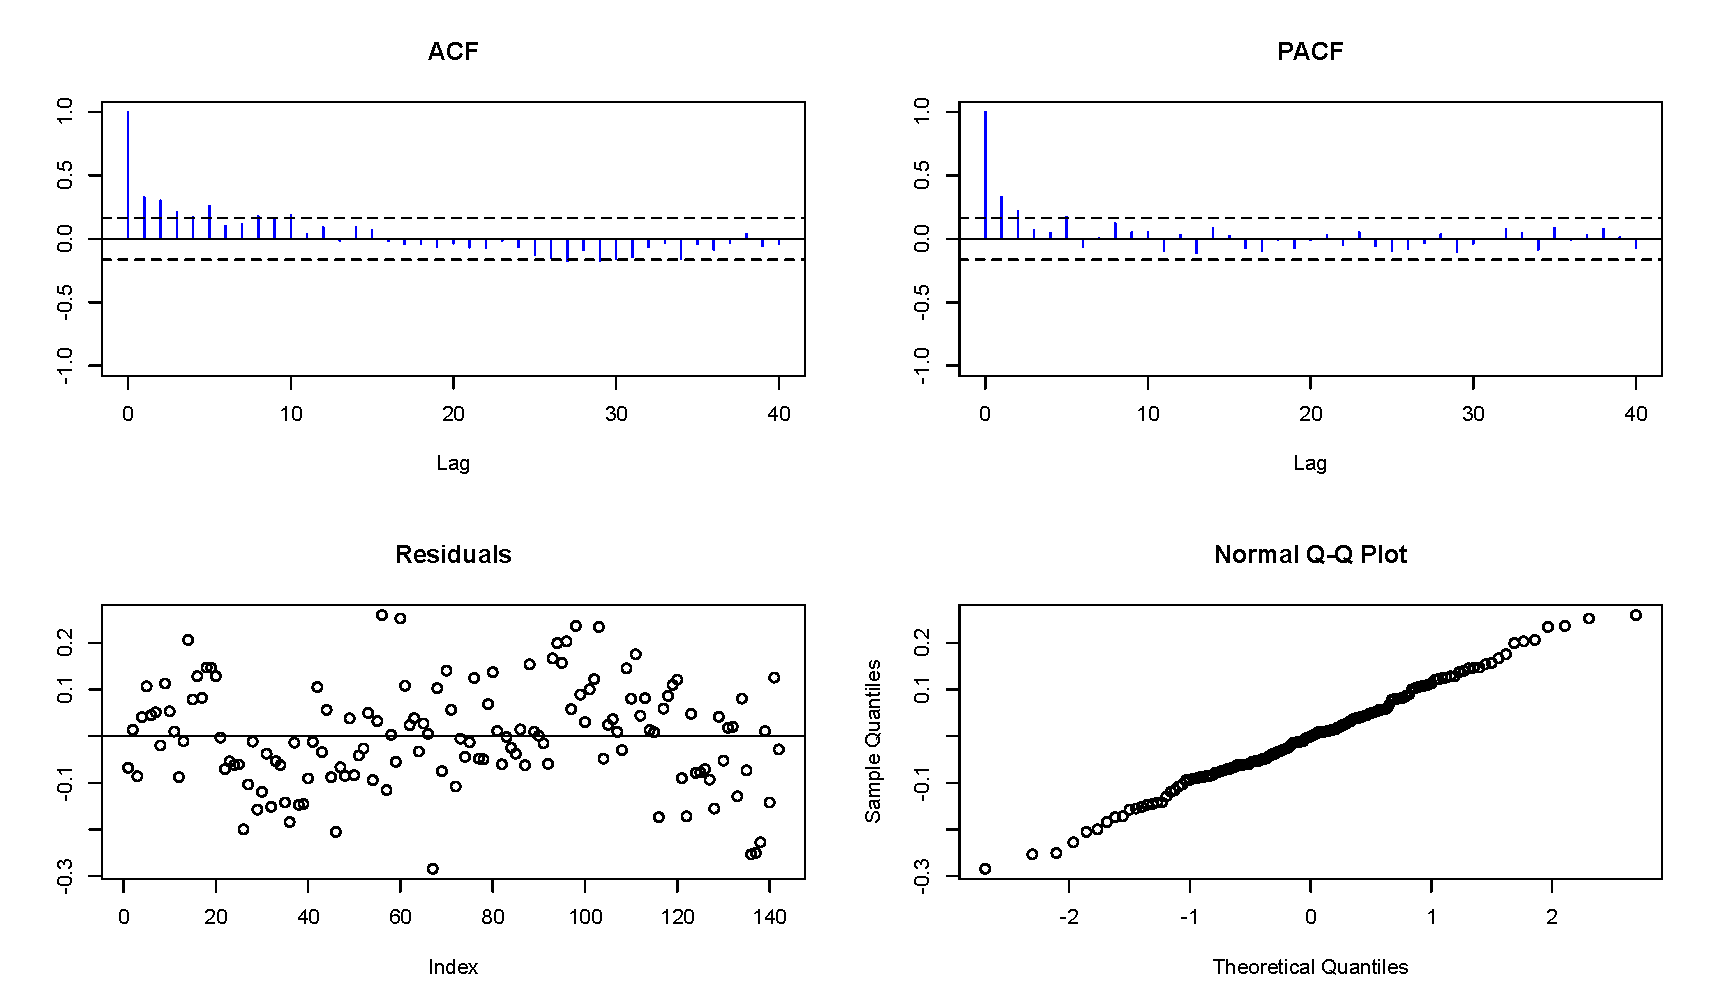
\includegraphics[scale=0.3]{Rplot-5.pdf}
\end{center}

\begin{verbatim}
Null hypothesis: Residuals are iid noise.
Test                        Distribution Statistic   p-value
Ljung-Box Q                Q ~ chisq(20)     71.57         0 *
McLeod-Li Q                Q ~ chisq(20)     12.07    0.9138
Turning points T     (T-93.3)/5 ~ N(0,1)        93    0.9468
Diff signs S       (S-70.5)/3.5 ~ N(0,1)        70    0.8848
Rank P         (P-5005.5)/283.5 ~ N(0,1)      5136    0.6453
\end{verbatim}

As seen above, the ACF and PACF plots decay rapidly indicating stationarity.
After $M$ is determined, the residuals of $M$ are
modeled with an ARMA model $a$.
In some circumstances
the following table can be useful for choosing $p$ and $q$ from the
plots of \verb$test(e)$.

\begin{center}
\begin{tabular}{|c|c|l|}
\hline
ACF & PACF & Model\\
\hline
Decays & Zero for $h>p$ & AR($p$)\\
Zero for $h>q$ & Decays & MA($q$)\\
Decays & Decays & ARMA($p$, $q$)\\
\hline
\end{tabular}
\end{center}

The ARMA model $a$ should yield residuals that resemble white noise.
To check for white noise, the {\tt test} function is used a second time.
The following is the result of $\tt test(ee)$ in the above example.

\begin{center}
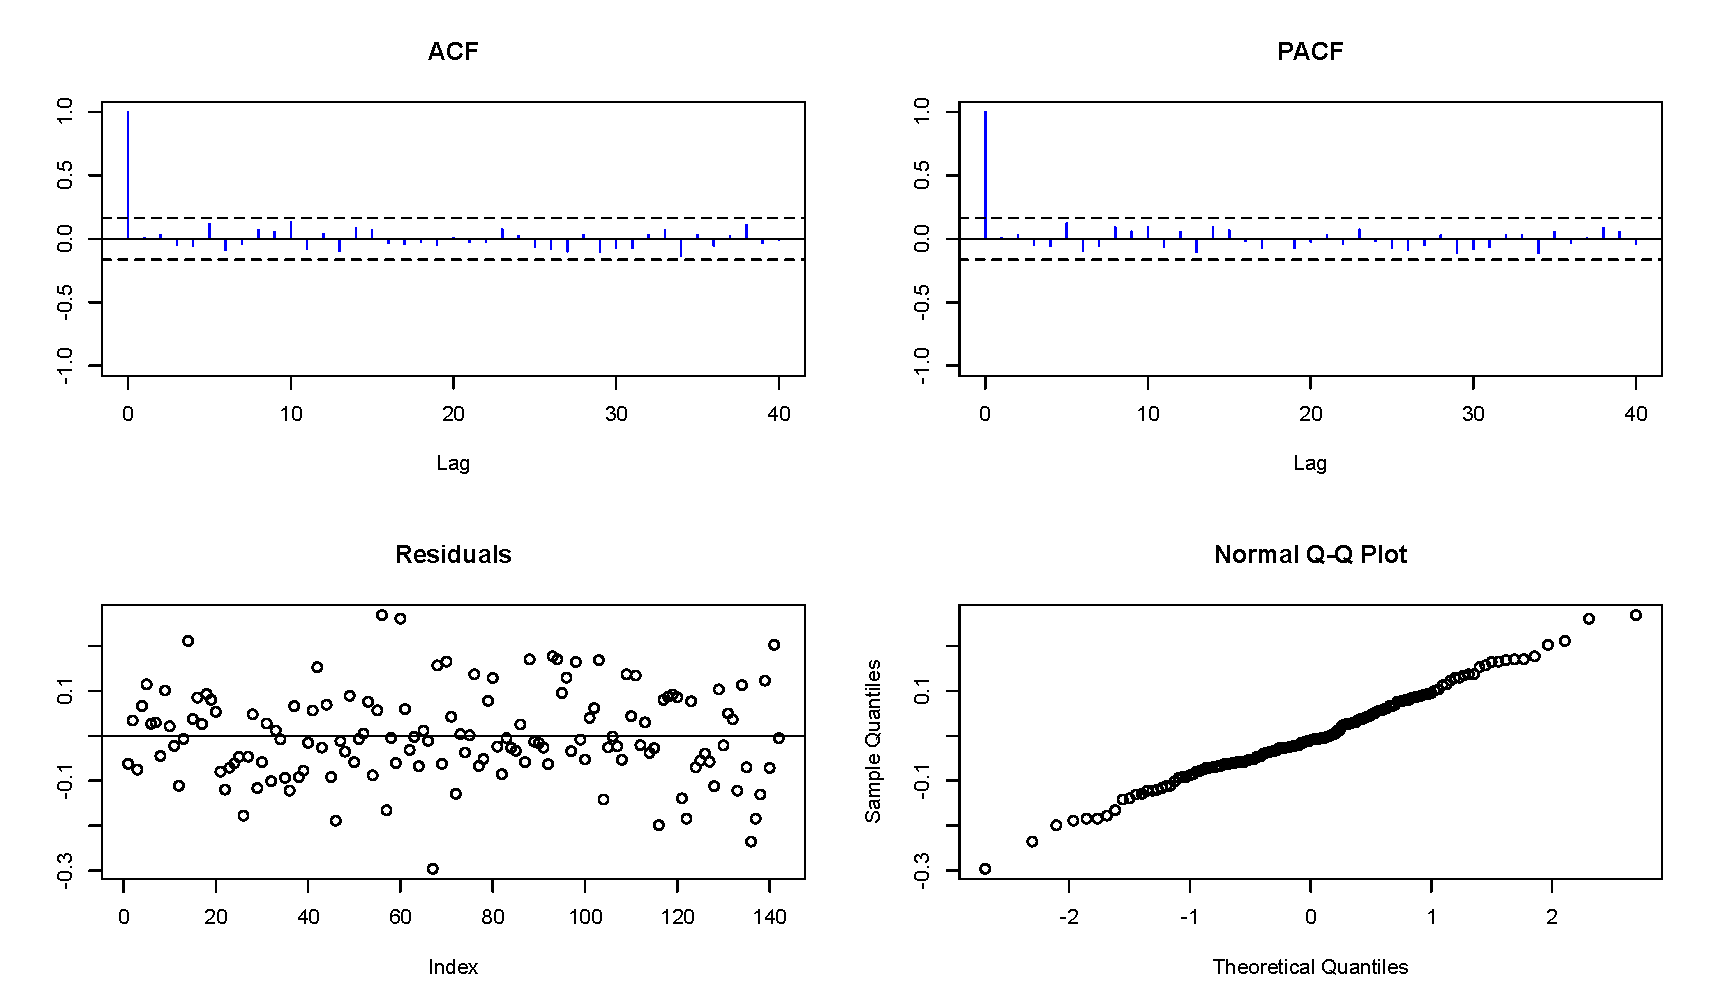
\includegraphics[scale=0.3]{Rplot-6.pdf}
\end{center}

\begin{verbatim}
Null hypothesis: Residuals are iid noise.
Test                        Distribution Statistic   p-value
Ljung-Box Q                Q ~ chisq(20)      13.3    0.8642
McLeod-Li Q                Q ~ chisq(20)     16.96    0.6556
Turning points T     (T-93.3)/5 ~ N(0,1)        93    0.9468
Diff signs S       (S-70.5)/3.5 ~ N(0,1)        70    0.8848
Rank P         (P-5005.5)/283.5 ~ N(0,1)      4999    0.9817
\end{verbatim}

The vertical lines in the ACF and PACF plots are below the noise threshold
(the dashed horizontal lines)
for lags greater than zero which is good.
In addition, the $p$-values in the table all fail to reject the null hypothesis
of iid noise.
Recall that a $p$-value is the probability that the null hypothesis is true.

\subsection{White Noise Variance}

ITSM-R includes five methods for estimating ARMA parameters.
They are Yule-Walker, Burg, Hannan-Rissanen, maximum likelihood,
and the innovations method.
For all estimation methods, ITSM-R uses
the following formula to estimate white noise variance
(Brockwell and Davis, page 164).
\[
\hat\sigma^2=\frac{1}{n}\sum_{t=1}^n\frac{(X_t-\hat X_t)^2}{r_{t-1}}
\]

The $X_t-\hat X_t$ are innovations (Brockwell and Davis, page 71).
Residuals are defined as follows (Brockwell and Davis, page 164).
\[
\hat W_t=\frac{X_t-\hat X_t}{\sqrt{r_{t-1}}}
\]

Thus $\hat\sigma^2$ is the average of the squared residuals.

\bigskip
The innovations algorithm (Brockwell and Davis, page 73)
is used to compute $\hat X_t$ and $r_{t-1}$.
Note that the algorithm produces mean squared errors
$v_{t-1}=E(X_t-\hat X_t)^2$ for $\kappa(i,j)=E(X_iX_j)$
given in equation (2.5.24).
However, ITSM-R uses $\kappa(i,j)=E(W_iW_j)$ given in
equation (3.3.3).
For the covariance in (3.3.3)
the innovations algorithm produces $r_{t-1}=E(W_t-\hat W_t)^2$
instead of $v_{t-1}$.
The relationship between $v_{t-1}$ and $r_{t-1}$ is given in
equation (3.3.8) as
\[
v_{t-1}=E(X_t-\hat X_t)^2=\sigma^2E(W_t-\hat W_t)^2=\sigma^2r_{t-1}
\]

where $\sigma^2$ is white noise variance.

\bigskip
It should be noted that $\gamma_X$ in (3.3.3) is
the autocovariance of the ARMA model, not of the data.
Then by equation (3.2.3) it can be seen that $\sigma^{-2}$ in (3.3.3)
cancels with $\sigma^2$ in $\gamma_X$.
Hence the innovations algorithm does not depend on white noise variance at all.
After the innovations are computed, white noise variance is estimated
using the above formula for $\hat\sigma^2$.
\begin{gather*}
\gamma_X(h)=E(X_{t+h}X_t)=\sigma^2\sum_{j=0}^\infty\psi_j\psi_{j+|h|}\tag{3.2.3}
\\
m=\max(p,q)\tag{3.3.2}
\\
\kappa(i,j)=\left\{
\begin{aligned}
&\sigma^{-2}\gamma_X(i-j), && 1\le i,\;j\le m\\
&\sigma^{-2}\left[
\gamma_X(i-j)-\sum_{r=1}^p\phi_r\gamma_X(r-|i-j|)\right],
&& \min(i,j)\le m<\max(i,j)\le2m,\\
&\sum_{r=0}^q\theta_r\theta_{r+|i-j|},&&\min(i,j)>m,\\
&0&&\text{otherwise.}
\end{aligned}
\right.\tag{3.3.3}
\end{gather*}

Because all estimation methods use the above formula for $\hat\sigma^2$,
variance estimates computed by ITSM-R are different from what is normally
expected.
For example, the Yule-Walker estimation function {\tt yw} returns a white noise
variance estimate that differs from the traditional Yule-Walker algorithm.

\bigskip
Since variance estimates are computed uniformly,
model AICCs can always be compared directly,
even when different methods are used to estimate model parameters.
For example, it is perfectly valid to compare the AICC of a Yule-Walker
model to that of a maximum likelihood model.

\subsection{ARMA Coefficients}
ARMA coefficient vectors are ordered such that
the vector index corresponds to the lag of the coefficient.
For example, the model
\[
X_t-\phi_1X_{t-1}-\phi_2X_{t-2}=Z_t+\theta_1Z_{t-1}+\theta_2Z_{t-2}
\]
with
\begin{align*}
\phi_1&=1/2\\
\phi_2&=1/3\\
\theta_1&=1/4\\
\theta_2&=1/5
\end{align*}
corresponds to the following R vectors.

\begin{verbatim}
phi = c(1/2,1/3)
theta = c(1/4,1/5)
\end{verbatim}

The equivalent model
\[
X_t=\phi_1X_{t-1}+\phi_2X_{t-2}
+Z_t+\theta_1Z_{t-1}+\theta_2Z_{t-2}
\]

makes plain the sign convention of the AR coefficients.

\subsection{ARIMA Models}
ARIMA($p$,$d$,$q$)
models are specified by differencing $d$ times with a lag of one each time.
For example, the following R code specifies an ARIMA(1,2,3) model
for data set {\tt quant}.

\begin{verbatim}
M = c("diff",1,"diff",1)
e = Resid(quant,M)
a = arma(e,1,3)
\end{verbatim}

\subsection{Data Sets}
ITSM-R includes the following data sets that are featured in
{\it Introduction to Time Series and Forecasting}.
Each data set is an ordinary vector (not a time series object).

\begin{center}
\begin{tabular}{|l|r|l|}
\hline
Name & Obs. & Description\\
\hline
{\tt airpass} & 144 & Number of international airline passengers, 1949 to 1960\\
{\tt deaths} & 72 & USA accidental deaths, 1973 to 1978\\
{\tt dowj} & 78 & Dow Jones utilities index, August 28 to December 18, 1972\\
{\tt lake} & 98 & Level of Lake Huron, 1875 to 1972\\
{\tt strikes} & 30 & USA union strikes, 1951 to 1980\\
{\tt Sunspots} & 100 & Number of sunspots, 1770 to 1869\\
{\tt wine} & 142 & Australian red wine sales, January 1980 to October 1991\\
\hline
\end{tabular}
\end{center}

\section{Functions}

\subsection{\tt aacvf}
Computes the autocovariance of an ARMA model.
\begin{flalign*}
\text{\tt aacvf(a,h)}\quad\left\{\begin{array}{ll}
{\tt a} & \text{ARMA model}\\
{\tt h} & \text{Maximum lag}
\end{array}\right.&&
\end{flalign*}

The ARMA model is a list with the following components.

\begin{quote}
\begin{tabular}{ll}
{\tt \$phi} & AR coefficients $\text{\tt[1:p]}=\phi_1,\ldots,\phi_p$\\
{\tt \$theta} & MA coefficients $\text{\tt[1:q]}=\theta_1,\ldots,\theta_q$\\
{\tt \$sigma2} & White noise variance $\sigma^2$
\end{tabular}
\end{quote}

Returns a vector of length {\tt h+1} to accomodate lag 0 at index 1.

\bigskip
The following example is from page 103 of
{\it Introduction to Time Series and Forecasting.}

\begin{verbatim}
R> a = specify(ar=c(1,-0.24),ma=c(0.4,0.2,0.1))
R> aacvf(a,3)
[1] 7.171327 6.441393 5.060274 3.614340
\end{verbatim}

\subsection{\tt acvf}
Computes the autocovariance of time series data.
\begin{flalign*}
\text{\tt acvf(x,h=40)}\quad\left\{\begin{array}{ll}
{\tt x} & \text{Time series data}\\
{\tt h} & \text{Maximum lag}
\end{array}\right.&&
\end{flalign*}

Returns a vector of length {\tt h+1} to accommodate lag 0
at index 1.

\bigskip
Example:

\begin{verbatim}
R> gamma = acvf(Sunspots)
R> plot(0:40,gamma,type="h")
\end{verbatim}

\begin{center}
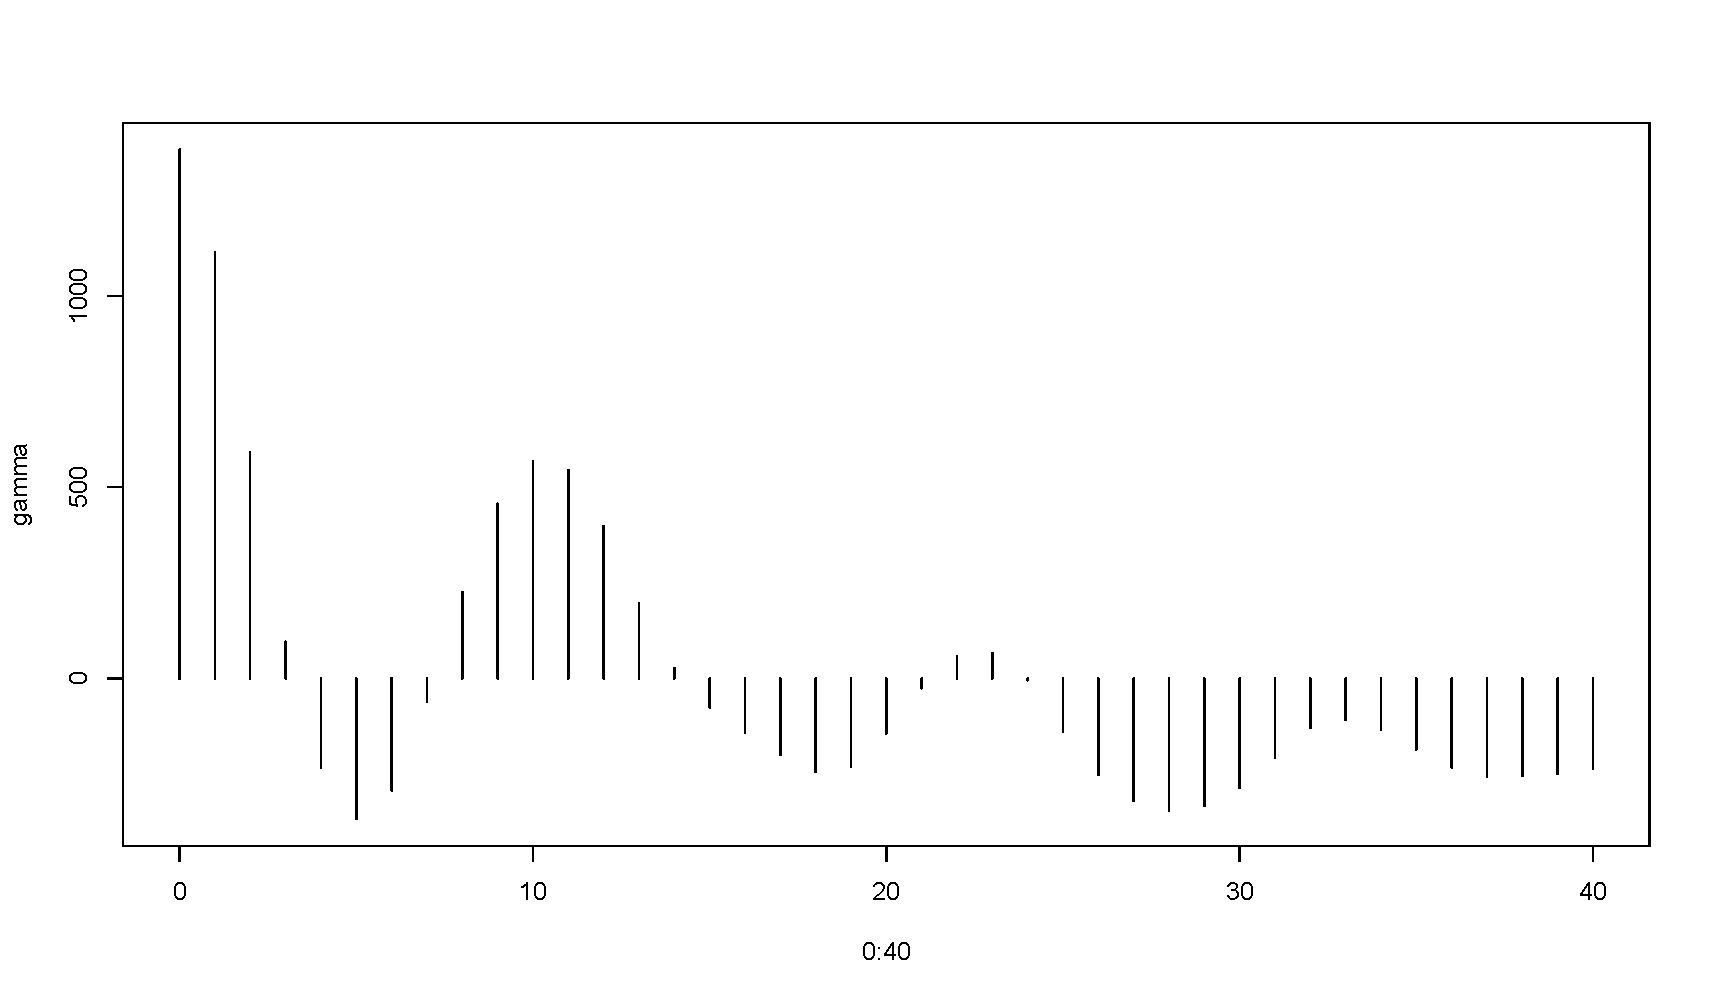
\includegraphics[scale=0.3]{Rplot-26.pdf}
\end{center}

\subsection{\tt ar.inf}
Returns the AR($\infty$) coefficients
$\pi_0$, $\pi_1$, $\ldots$, $\pi_n$ where $\pi_0=1$.
\begin{flalign*}
\text{\tt ar.inf(a,n)}\quad\left\{\begin{array}{ll}
{\tt a} & \text{ARMA model}\\
{\tt n} & \text{Order}
\end{array}\right.&&
\end{flalign*}

A vector of length {\tt n+1} is returned to accommodate $\pi_0$ at index 1.

\bigskip
Example:

\begin{verbatim}
R> a = yw(Sunspots,2)
R> ar.inf(a,10)
 [1]  1.0000000 -1.3175005  0.6341215  0.0000000  0.0000000  0.0000000
 [7]  0.0000000  0.0000000  0.0000000  0.0000000  0.0000000
\end{verbatim}

\bigskip
For invertible ARMA processes,
AR($\infty$) is the polynomial $\pi(z)$ such that
\[
\pi(z)=\frac{\phi(z)}{\theta(z)}=1+\pi_1z+\pi_2z^2+\cdots
\]
The corresponding autoregression is
\[
Z_t=\pi(B)X_t=X_t+\pi_1X_{t-1}+\pi_2X_{t-2}+\cdots
\]
The coefficients $\pi_j$ are calculated recursively using the following formula.
(See page 86 of {\it Introduction to Time Series and Forecasting.})
\[
\pi_j=-\phi_j-\sum_{k=1}^q\theta_k\pi_{j-k}\qquad j=1,2,\ldots
\]

\subsection{\tt arar}
Predict future values of a time series using the ARAR algorithm.
\begin{flalign*}
\text{\tt arar(x,h=10,opt=2)}\quad\left\{\begin{array}{ll}
{\tt x} & \text{Observed data}\\
{\tt h} & \text{Steps ahead}\\
{\tt opt} & \text{Display option}
\end{array}\right.&&
\end{flalign*}

The display options are 0 for silent, 1 for tabulate, 2 for plot and tabulate.
Returns the following list invisibly.

\begin{quote}
\begin{tabular}{ll}
{\tt\$pred} & Predicted values\\
{\tt\$se} & Standard errors\\
{\tt\$l} & Lower bounds\\
{\tt\$u} & Upper bounds
\end{tabular}
\end{quote}

Example:

\begin{verbatim}
R> arar(airpass)
Optimal lags 1 2 9 10 
Optimal coeffs 0.5247184 0.2735903 0.2129203 -0.316453 
WN Variance 110.1074 
Filter 1 -0.5247184 -0.2735903 0 0 0 0 0 0 -0.2129203 0.316453 0
-1.114253 0.5846688 0.3048487 0 0 0 0 0 0 0.237247 -0.3526086 
 Step     Prediction      sqrt(MSE)    Lower Bound    Upper Bound
    1       466.1915       10.49321       445.6248       486.7582
    2       426.3592       11.85003       403.1331       449.5853
    3        463.614       13.17574       437.7895       489.4384
    4       509.5108       13.93231       482.2035       536.8182
    5       516.2016       14.48202       487.8169       544.5864
    6       594.0837       14.85609       564.9658       623.2017
    7       693.9735       15.12129       664.3358       723.6112
    8       670.4816       15.30835       640.4772       700.4859
    9       564.4617       15.44148       534.1964        594.727
   10       518.5135       15.93834       487.2743       549.7526
\end{verbatim}

\begin{center}
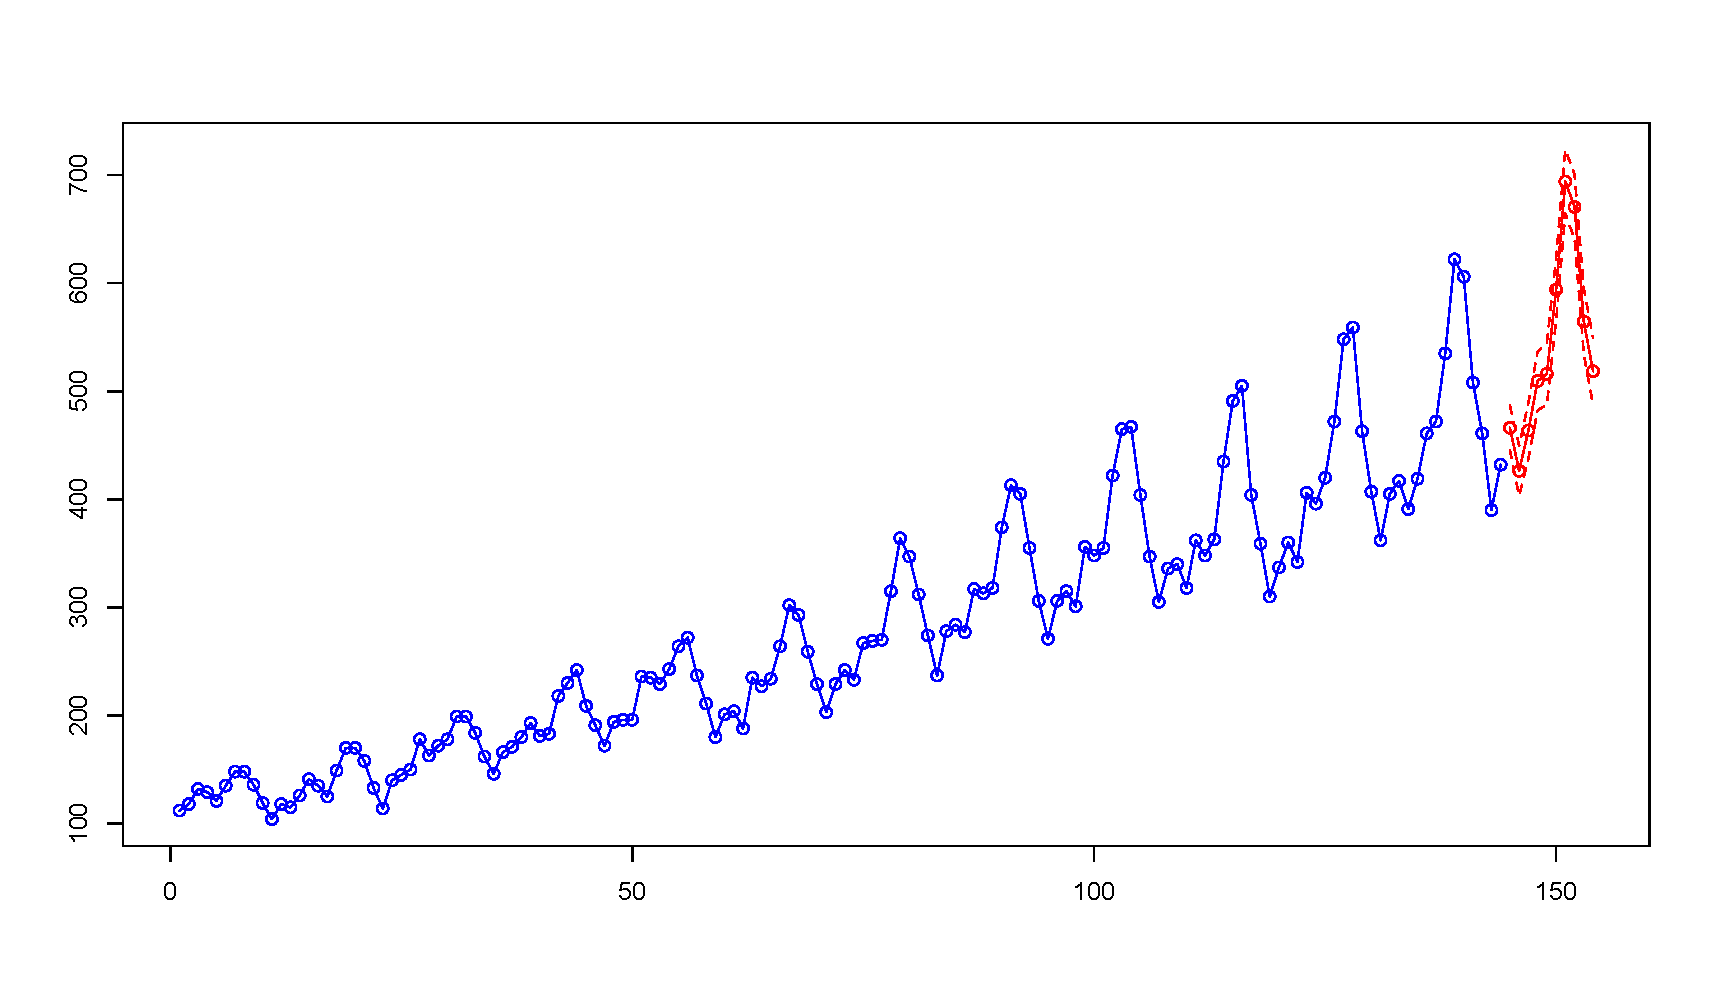
\includegraphics[scale=0.3]{Rplot-4.pdf}
\end{center}

\subsection{\tt arma}
Returns an ARMA model using maximum likelihood
to estimate the AR and MA coefficients.
\begin{flalign*}
\text{\tt arma(x,p=0,q=0)}\quad\left\{\begin{array}{ll}
{\tt x} & \text{Time series data}\\
{\tt p} & \text{AR order}\\
{\tt q} & \text{MA order}
\end{array}\right.&&
\end{flalign*}

The R function {\tt arima} is called to
estimate $\phi$ and $\theta$.
The innovations algorithm is used to estimate the white noise
variance $\sigma^2$.
The resulting ARMA model is a list with the following components.

\begin{quote}
\begin{tabular}{ll}
{\tt \$phi} & AR coefficients $\text{\tt[1:p]}=\phi_1,\ldots,\phi_p$\\
{\tt \$theta} & MA coefficients $\text{\tt[1:q]}=\theta_1,\ldots,\theta_q$\\
{\tt \$sigma2} & White noise variance $\sigma^2$\\
{\tt \$aicc} & Akaike information criterion corrected\\
{\tt \$se.phi} & Standard errors for the AR coefficients\\
{\tt \$se.theta} & Standard errors for the MA coefficients
\end{tabular}
\end{quote}

The signs of the coefficients correspond to the following model.
\[
X_t=\sum_{j=1}^p\phi_jX_{t-j}+Z_t+\sum_{k=1}^q\theta_kZ_{t-k}
\]

The following example estimates ARMA(1,0) parameters
for a stationary transformation of the Dow Jones data.

\begin{verbatim}
R> M = c("diff",1)
R> e = Resid(dowj,M)
R> a = arma(e,1,0)
R> a
$phi
[1] 0.4478187

$theta
[1] 0

$sigma2
[1] 0.1455080

$aicc
[1] 74.48316

$se.phi
[1] 0.01105692

$se.theta
[1] 0
\end{verbatim}

\subsection{\tt autofit}
Uses maximum likelihood to determine the best ARMA model given a range of models.
The {\tt autofit} function tries all combinations of argument sequences and returns the model
with the lowest AICC.
This is a wrapper function,
the R function {\tt arima} does
the actual estimation.
\begin{flalign*}
\text{\tt autofit(x,p=0:5,q=0:5)}\quad\left\{\begin{array}{ll}
{\tt x} & \text{Time series data}\\
{\tt p} & \text{AR order}\\
{\tt q} & \text{MA order}
\end{array}\right.&&
\end{flalign*}

Returns a list with the following components.

\begin{quote}
\begin{tabular}{ll}
{\tt \$phi} & AR coefficients $\text{\tt[1:p]}=\phi_1,\ldots,\phi_p$\\
{\tt \$theta} & MA coefficients $\text{\tt[1:q]}=\theta_1,\ldots,\theta_q$\\
{\tt \$sigma2} & White noise variance $\sigma^2$\\
{\tt \$aicc} & Akaike information criterion corrected\\
{\tt \$se.phi} & Standard errors for the AR coefficients\\
{\tt \$se.theta} & Standard errors for the MA coefficients
\end{tabular}
\end{quote}

The signs of the coefficients correspond to the following model.
\[
X_t=\sum_{j=1}^p\phi_jX_{t-j}+Z_t+\sum_{k=1}^q\theta_kZ_{t-k}
\]

The following example shows that an ARMA(1,1) model has the lowest AICC
for the Lake Huron data.

\begin{verbatim}
R> autofit(lake)
$phi
[1] 0.7448993

$theta
[1] 0.3205891

$sigma2
[1] 0.4750447

$aicc
[1] 212.7675

$se.phi
[1] 0.006029624

$se.theta
[1] 0.01288894
\end{verbatim}

\subsection{\tt burg}
Estimates AR coefficients using the Burg method.
\begin{flalign*}
\text{\tt burg(x,p)}\quad\left\{\begin{array}{ll}
{\tt x} & \text{Time series data}\\
{\tt p} & \text{AR order}
\end{array}\right.&&
\end{flalign*}

Returns an ARMA model with the following components.

\begin{quote}
\begin{tabular}{ll}
{\tt \$phi} & AR coefficients $\text{\tt[1:p]}=\phi_1,\ldots,\phi_p$\\
{\tt \$theta} & 0\\
{\tt \$sigma2} & White noise variance $\sigma^2$\\
{\tt \$aicc} & Akaike information criterion corrected\\
{\tt \$se.phi} & Standard errors for AR coefficients\\
{\tt \$se.theta} & 0
\end{tabular}
\end{quote}

Example:
\begin{verbatim}
R> burg(lake,1)
$phi
[1] 0.8388953

$theta
[1] 0

$sigma2
[1] 0.5096105

$aicc
[1] 217.3922

$se.phi
[1] 0.003023007

$se.theta
[1] 0
\end{verbatim}

\subsection{\tt check}
Check for causality and invertibility of an ARMA model.
\begin{flalign*}
\text{\tt check(a)}\quad\left\{\begin{array}{ll}
{\tt a} & \text{ARMA model}\\
\end{array}\right.&&
\end{flalign*}

The ARMA model is a list with the following components.

\begin{quote}
\begin{tabular}{ll}
{\tt \$phi} & AR coefficients $\text{\tt[1:p]}=\phi_1,\ldots,\phi_p$\\
{\tt \$theta} & MA coefficients $\text{\tt[1:q]}=\theta_1,\ldots,\theta_q$
\end{tabular}
\end{quote}

Example:
\begin{verbatim}
R> a = specify(ar=c(0,0,0.99))
R> check(a)
Causal
Invertible
\end{verbatim}

\subsection{\tt forecast}
Predict future values of a time series.
\begin{flalign*}
\text{\tt forecast(x,M,a,h=10,opt=2,alpha=0.05)}\quad\left\{\begin{array}{ll}
{\tt x} & \text{Time series data}\\
{\tt M} & \text{Data model}\\
{\tt a} & \text{ARMA model}\\
{\tt h} & \text{Steps ahead}\\
{\tt opt} & \text{Display option}\\
{\tt alpha} & \text{Level of significance}
\end{array}\right.&&
\end{flalign*}

The data model {\tt M} can be {\tt NULL} for none.
The display options are 0 for none, 1 for tabulate,
2 for plot and tabulate.
See below for details about the data model.

\bigskip
Example:

\begin{verbatim}
R> M = c("log","season",12,"trend",1)
R> e = Resid(wine,M)
R> a = arma(e,1,1)
R> forecast(wine,M,a)
 Step     Prediction    Lower Bound    Upper Bound
    1       2227.556       1834.156       2705.334
    2       2374.062       1946.145       2896.069
    3       1216.429        993.925       1488.743
    4       1634.838       1332.583       2005.651
    5       1883.996       1532.926       2315.467
    6       2097.927       1704.717       2581.833
    7       2524.942       2049.658       3110.437
    8       2542.990       2062.775       3135.001
    9       3096.280       2510.185       3819.219
   10       3180.418       2577.324       3924.636
\end{verbatim}

\begin{center}
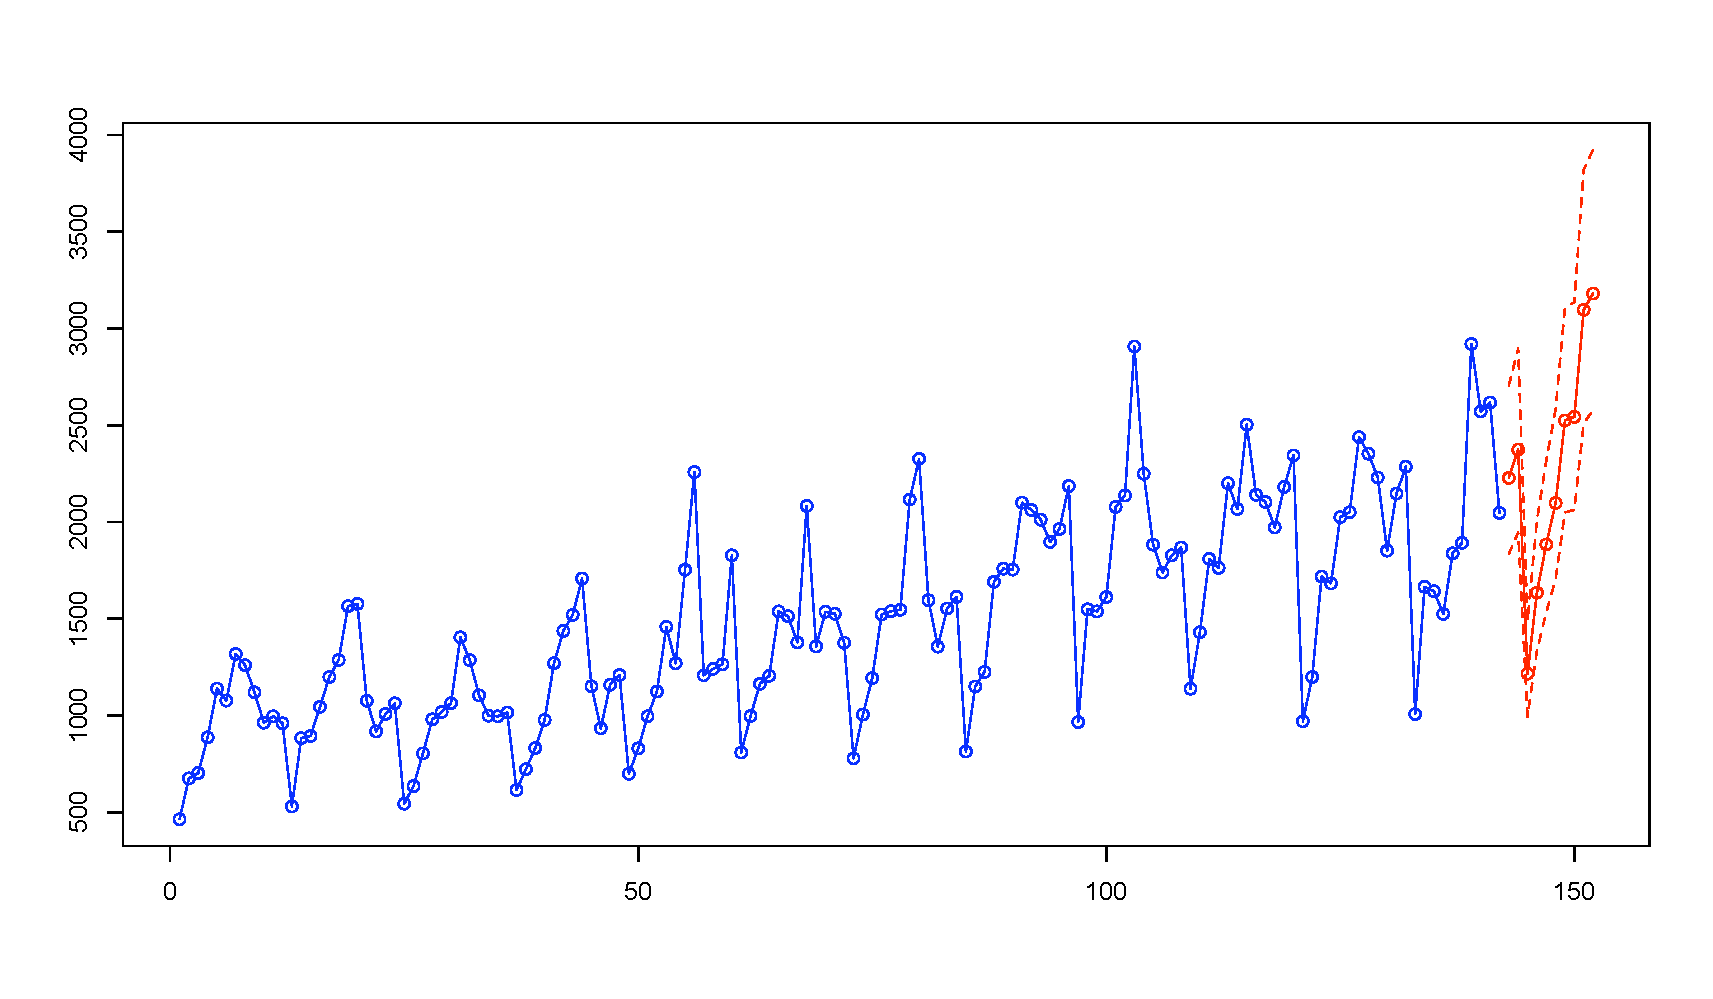
\includegraphics[scale=0.3]{Rplot-34.pdf}
\end{center}

The data model {\tt M} is a vector of function names.
The functions are applied to the data in left to right order.
There are five functions from which to choose.

\begin{quote}
\begin{tabular}{ll}
{\tt diff} & Difference the data\\
{\tt hr} & Subtract harmonic components\\
{\tt log} & Take the log of the data\\
{\tt season} & Subtract seasonal component\\
{\tt trend} & Subtract trend component\\
\end{tabular}
\end{quote}

A function name may be followed by one or more arguments.

\bigskip
{\tt diff} has a single argument, the lag.

\bigskip
{\tt hr} has one or more arguments, each specifying the number
of observations per harmonic period.

\bigskip
{\tt log} has no arguments.

\bigskip
{\tt season} has one argument, the number of observations per season.

\bigskip
{\tt trend} has one argument, the polynomial order of the trend,
(1 for linear, 2 for quadratic, etc.)

\bigskip
A data model is built up by concatenating the function
names and arguments. For example, the following vector takes the
log of the data, then subtracts a seasonal component of period twelve
then subtracts a linear trend component.

\begin{verbatim}
R> M = c("log","season",12,"trend",1)
\end{verbatim}

At the end of the data model there is an implied subtraction
of the mean operation.
Hence the resulting time series always has zero mean.

\subsection{\tt hannan}
Estimates ARMA coefficients using the Hannan-Rissanen algorithm.
It is required that $q>0$.
\begin{flalign*}
\text{\tt hannan(x,p,q)}\quad\left\{\begin{array}{ll}
{\tt x} & \text{Time series data}\\
{\tt p} & \text{AR order}\\
{\tt q} & \text{MA order}
\end{array}\right.&&
\end{flalign*}

Returns a list with the following components.

\begin{quote}
\begin{tabular}{ll}
{\tt \$phi} & AR coefficients $\text{\tt[1:p]}=\phi_1,\ldots,\phi_p$\\
{\tt \$theta} & MA coefficients $\text{\tt[1:q]}=\theta_1,\ldots,\theta_q$\\
{\tt \$sigma2} & White noise variance $\sigma^2$\\
{\tt \$aicc} & Akaike information criterion corrected\\
{\tt \$se.phi} & Standard errors for AR coefficients\\
{\tt \$se.theta} & Standard errors for MA coefficients
\end{tabular}
\end{quote}

Example:
\begin{verbatim}
R> hannan(lake,1,1)
$phi
[1] 0.6960772

$theta
[1] 0.3787969

$sigma2
[1] 0.477358

$aicc
[1] 213.183

$se.phi
[1] 0.07800321

$se.theta
[1] 0.1465265
\end{verbatim}

\subsection{\tt hr}
Returns the sum of harmonic components of time series data.
\begin{flalign*}
\text{\tt hr(x,d)}\quad\left\{\begin{array}{ll}
{\tt x} & \text{Time series data}\\
{\tt d} & \text{Vector of harmonic periods}
\end{array}\right.&&
\end{flalign*}

Example:
\begin{verbatim}
R> y = hr(deaths,c(12,6))
R> plotc(deaths,y)
\end{verbatim}

\begin{center}
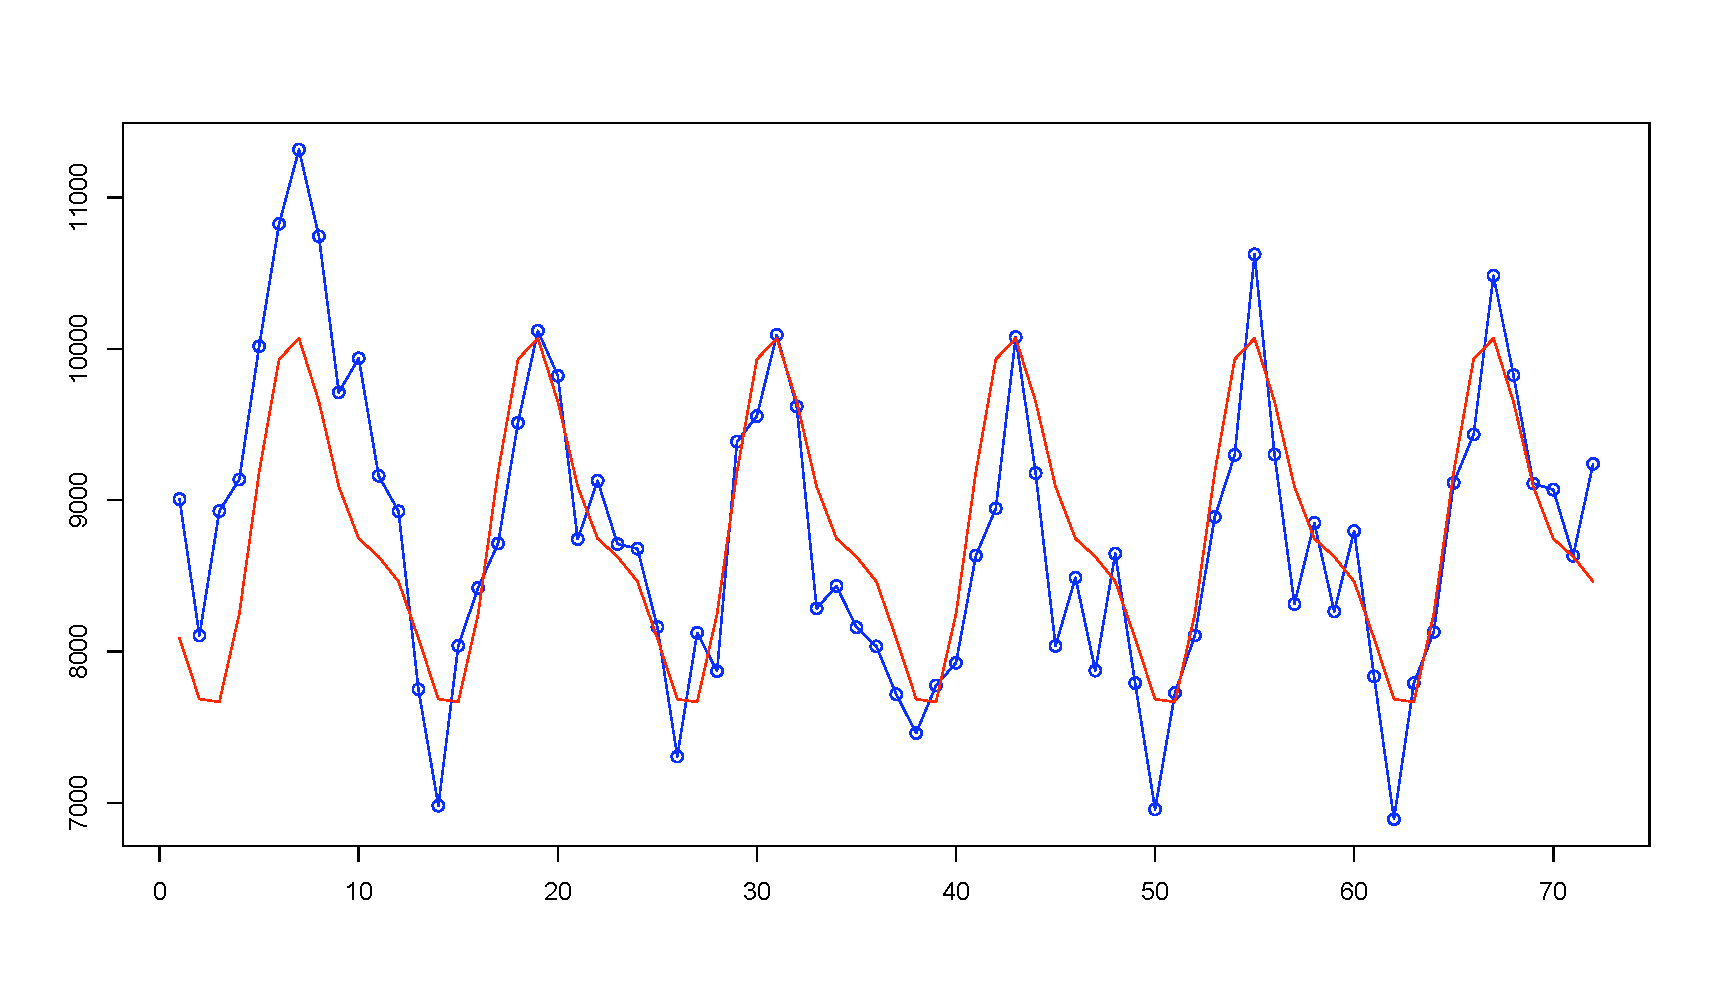
\includegraphics[scale=0.3]{Rplot-12.pdf}
\end{center}

\subsection{\tt ia}
Calculates MA coefficients using the innovations algorithm.
\begin{flalign*}
\text{\tt ia(x,q,m=17)}\quad\left\{\begin{array}{ll}
{\tt x} & \text{Time series data}\\
{\tt q} & \text{MA order}\\
{\tt m} & \text{Recursion level}
\end{array}\right.&&
\end{flalign*}

Returns a list with the following components.

\begin{quote}
\begin{tabular}{ll}
{\tt \$phi} & 0\\
{\tt \$theta} & MA coefficients $\text{\tt[1:q]}=\theta_1,\ldots,\theta_q$\\
{\tt \$sigma2} & White noise variance $\sigma^2$\\
{\tt \$aicc} & Akaike information criterion corrected\\
{\tt \$se.phi} & 0\\
{\tt \$se.theta} & Standard errors for MA coefficients
\end{tabular}
\end{quote}

Normally {\tt m} should be set to the default 17 even when fewer MA coefficients
are required.

\bigskip
The following example generates results that match
{\it Introduction to Time Series and Forecasting} page 154.
\begin{verbatim}
R> y = diff(dowj)
R> a = ia(y,17)
R> round(a$theta,4)
 [1]  0.4269  0.2704  0.1183  0.1589  0.1355  0.1568  0.1284 -0.0060
 [9]  0.0148 -0.0017  0.1974 -0.0463  0.2023  0.1285 -0.0213 -0.2575
[17]  0.0760
R> round(a$theta/a$se/1.96,4)
 [1]  1.9114  1.1133  0.4727  0.6314  0.5331  0.6127  0.4969 -0.0231
 [9]  0.0568 -0.0064  0.7594 -0.1757  0.7666  0.4801 -0.0792 -0.9563
[17]  0.2760
\end{verbatim}

The formula for the standard error of the $j$th coefficient is given
on page 152 of {\it Introduction to Time Series and Forecasting} as
\[
\sigma_j=n^{-1/2}\left[\sum_{i=0}^{j-1}\hat\theta_{mi}^2\right]^{1/2}
\]
where $\hat\theta_{m0}=1$.
Hence the standard error for $\hat\theta_1$ is $\sigma_1=n^{-1/2}$.

\subsection{\tt ma.inf}
Returns the MA($\infty$) coefficients
$\psi_0$, $\psi_1$, $\ldots$, $\psi_n$ where $\psi_0=1$.
\begin{flalign*}
\text{\tt ma.inf(m,n)}\quad\left\{\begin{array}{ll}
{\tt a} & \text{ARMA model}\\
{\tt n} & \text{Order}
\end{array}\right.&&
\end{flalign*}

A vector of length {\tt n+1} is returned to accommodate $\psi_0$ at index 1.

\bigskip
Example:

\begin{verbatim}
R> a = yw(Sunspots,2)
R> ma.inf(a,10)
 [1]  1.00000000  1.31750053  1.10168617  0.61601672  0.11299949
 [6] -0.24175256 -0.39016452 -0.36074148 -0.22786538 -0.07145884
[11]  0.05034727
\end{verbatim}

\bigskip
For causal ARMA processes,
MA($\infty$) is the polynomial $\psi(z)$ such that
\[
\psi(z)=\frac{\theta(z)}{\phi(z)}=1+\psi_1z+\psi_2z^2+\cdots
\]
The corresponding moving average is
\[
X_t=\psi(B)Z_t=Z_t+\psi_1Z_{t-1}+\psi_2Z_{t-2}+\cdots
\]
The coefficients $\psi_j$ are calculated recursively using the following formula.
(See page 85 of {\it Introduction to Time Series and Forecasting.})
\[
\psi_j=
\theta_j+\sum_{k=1}^p\phi_k\psi_{j-k}\qquad j=1,2,\ldots
\]

\subsection{\tt periodogram}
Plots a periodogram.
\begin{flalign*}
\text{\tt periodogram(x,q=0,opt=2)}\quad\left\{\begin{array}{ll}
{\tt x} & \text{Time series data}\\
{\tt q} & \text{MA filter order}\\
{\tt opt} & \text{Plot option}
\end{array}\right.&&
\end{flalign*}

The periodogram vector divided by $2\pi$ is returned invisibly.
The plot options are 0 for no plot, 1 to plot only the periodogram,
and 2 to plot both the periodogram and the filter coefficients.
The filter {\tt q} can be a vector in which case the overall filter is the
composition of MA filters of the designated orders.

\begin{verbatim}
R> periodogram(Sunspots,c(1,1,1,1))
Filter  0.01234568 0.04938272 0.1234568 0.1975309 0.2345679 0.1975309
 0.1234568 0.04938272 0.01234568 
\end{verbatim}

\begin{center}
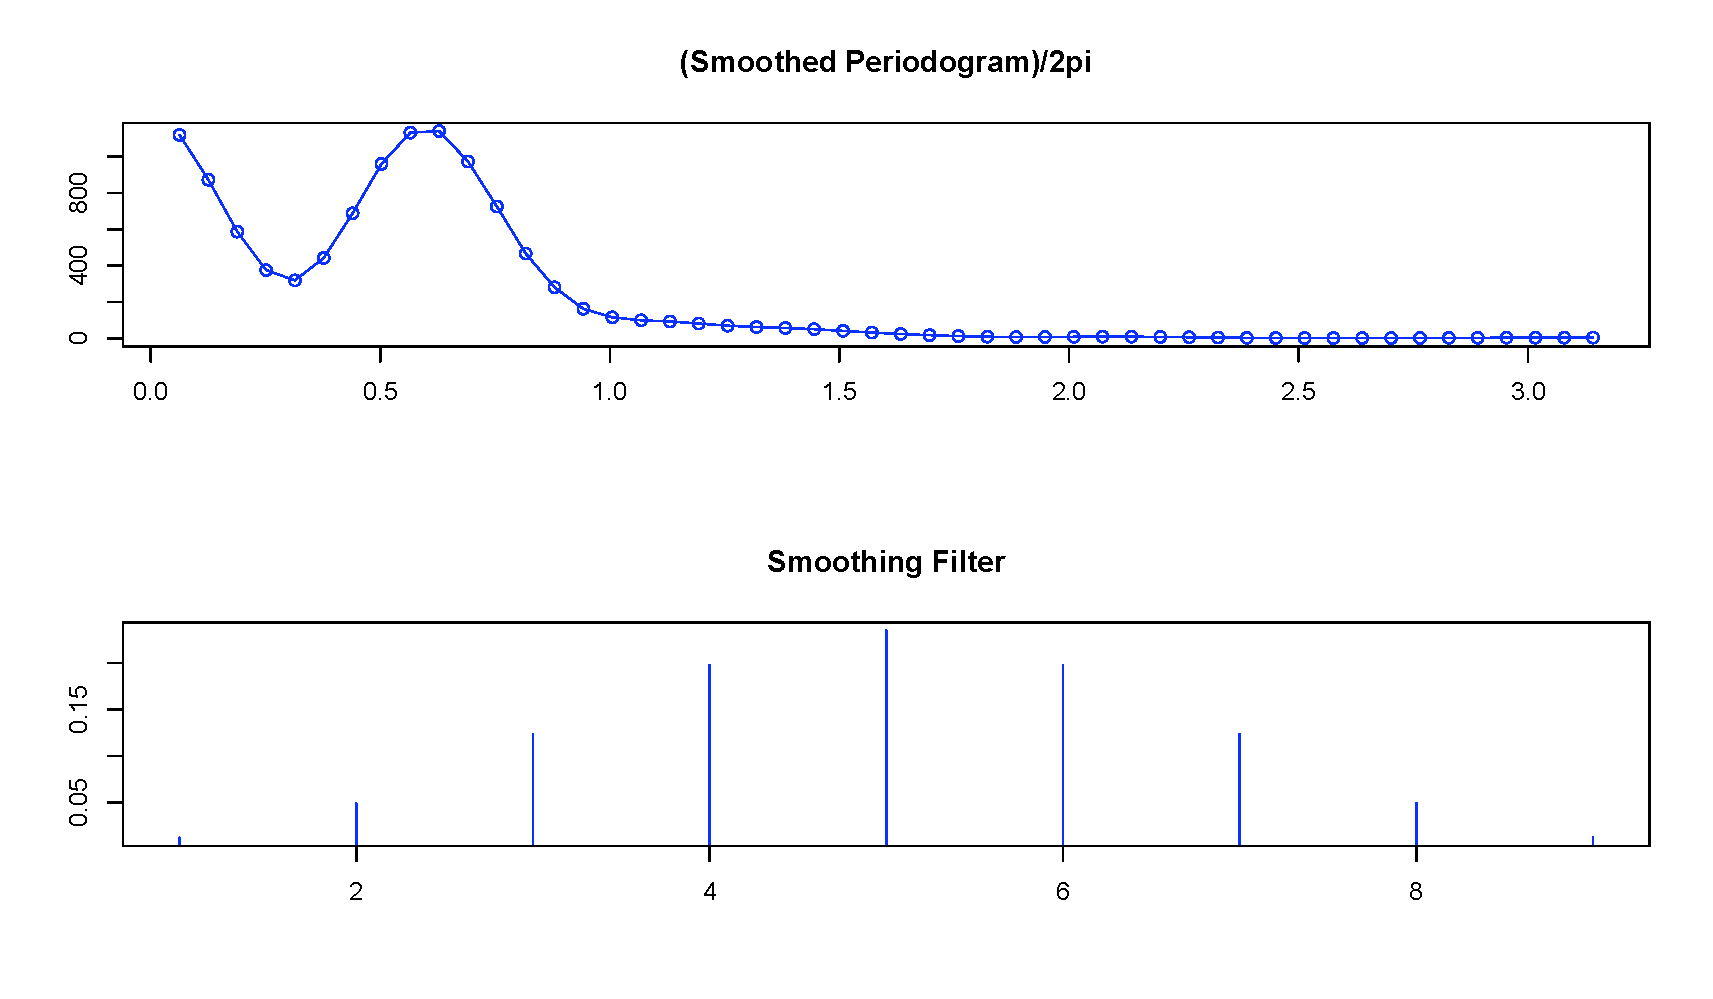
\includegraphics[scale=0.3]{Rplot-52.pdf}
\end{center}

\subsection{\tt plota}
Plots ACF and PACF for time series data and/or ARMA model.
\begin{flalign*}
\text{\tt plota(u,v=NULL,h=40)}\quad\left\{\begin{array}{ll}
{\tt u, v} & \text{Time series data and/or ARMA model, in either order}\\
{\tt h} & \text{Maximum lag}
\end{array}\right.&&
\end{flalign*}

Example:

\begin{verbatim}
R> plota(Sunspots)
\end{verbatim}

\begin{center}
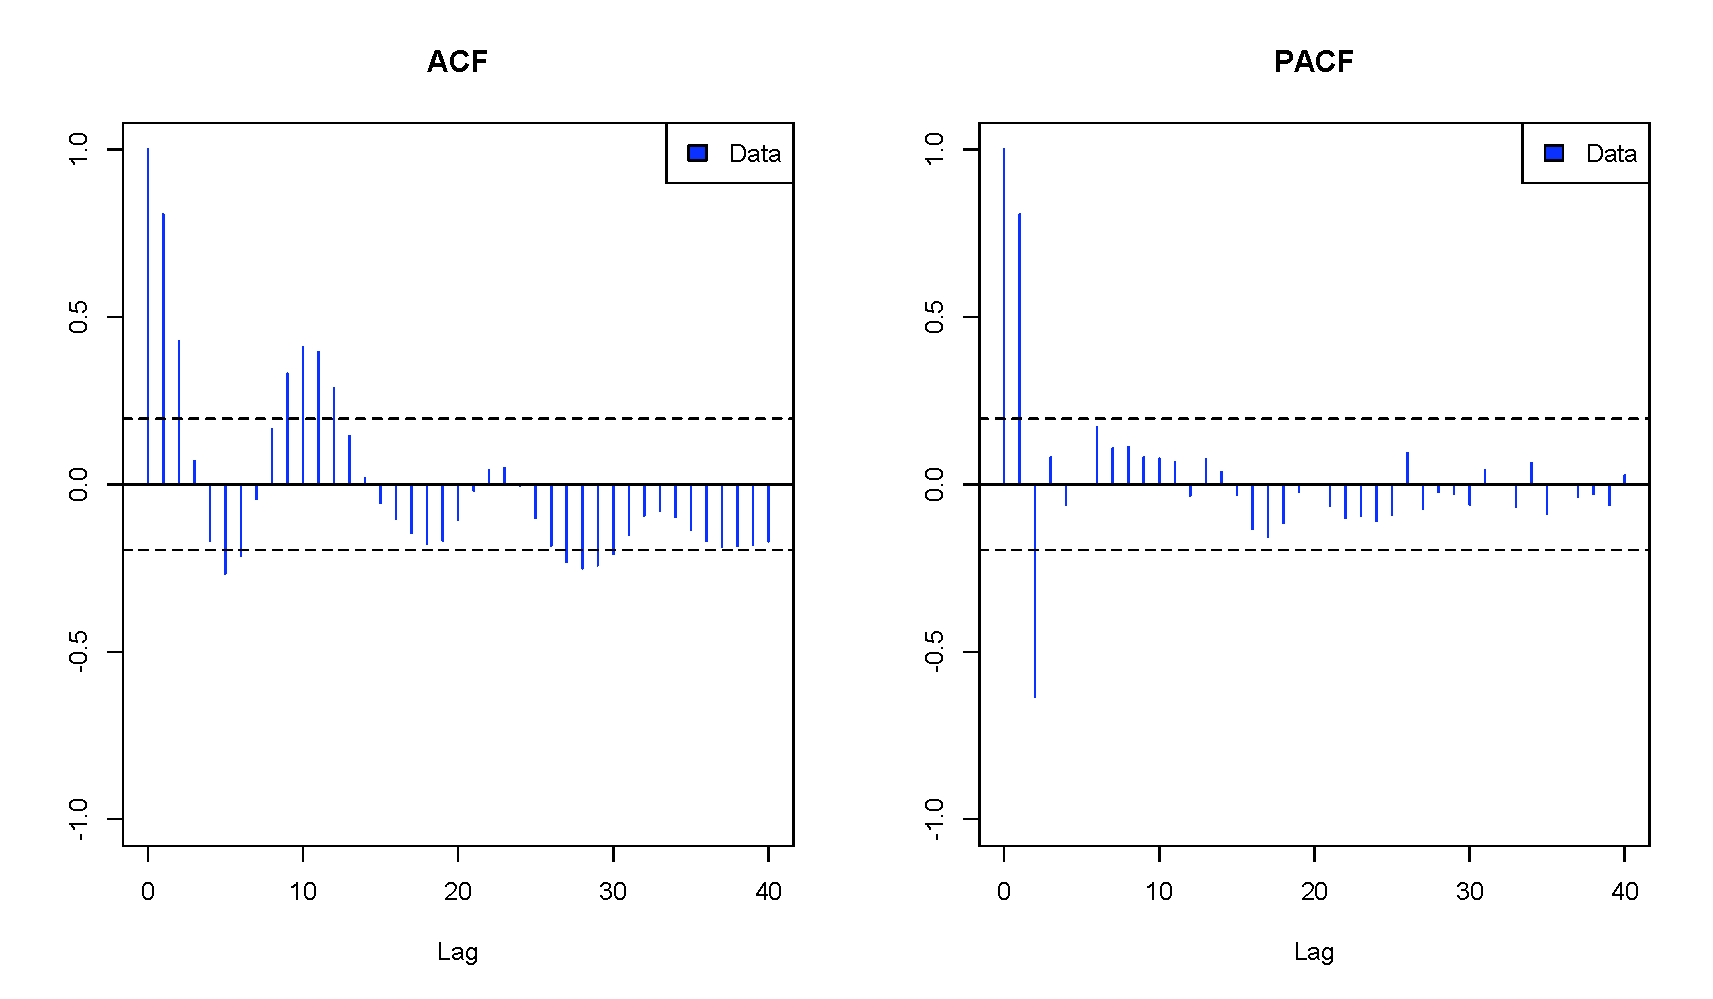
\includegraphics[scale=0.3]{Rplot-21.pdf}
\end{center}

\begin{verbatim}
R> a = yw(Sunspots,2)
R> plota(Sunspots,a)
\end{verbatim}

\begin{center}
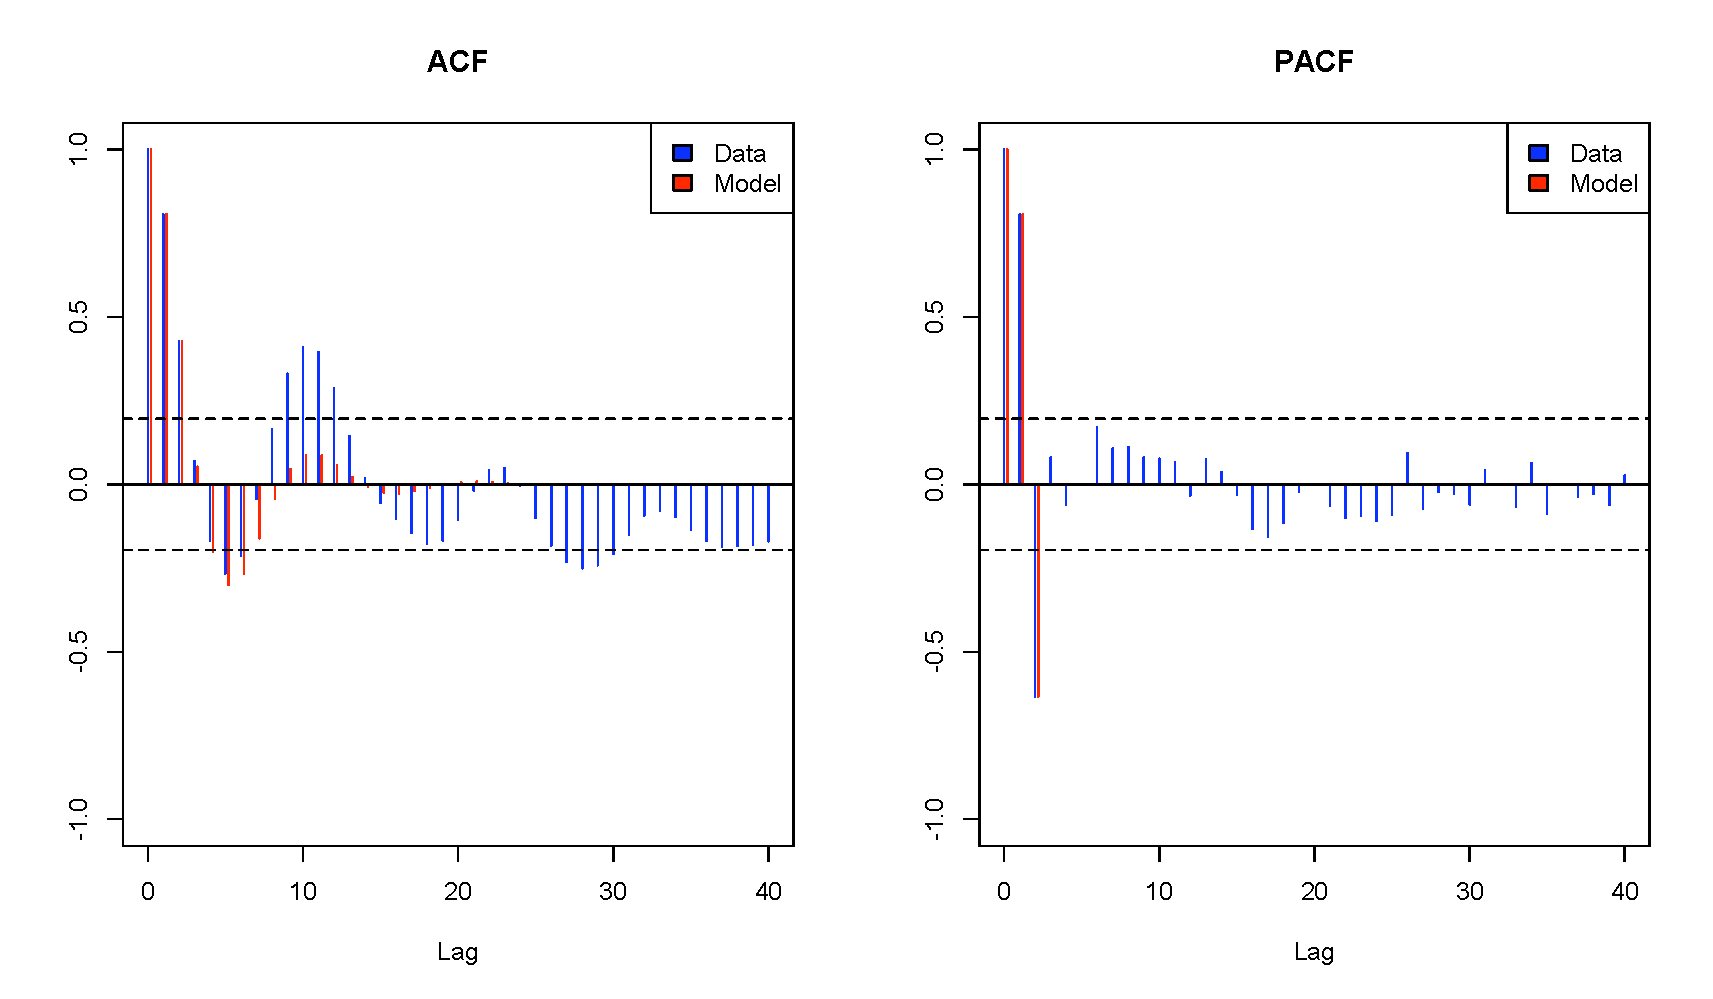
\includegraphics[scale=0.3]{Rplot-22.pdf}
\end{center}

The following example demonstrates the utility of the $\pm1.96/\sqrt{n}$ bounds
as a test for noise.

\begin{verbatim}
R> noise = rnorm(200)
R> plota(noise)
\end{verbatim}

\begin{center}
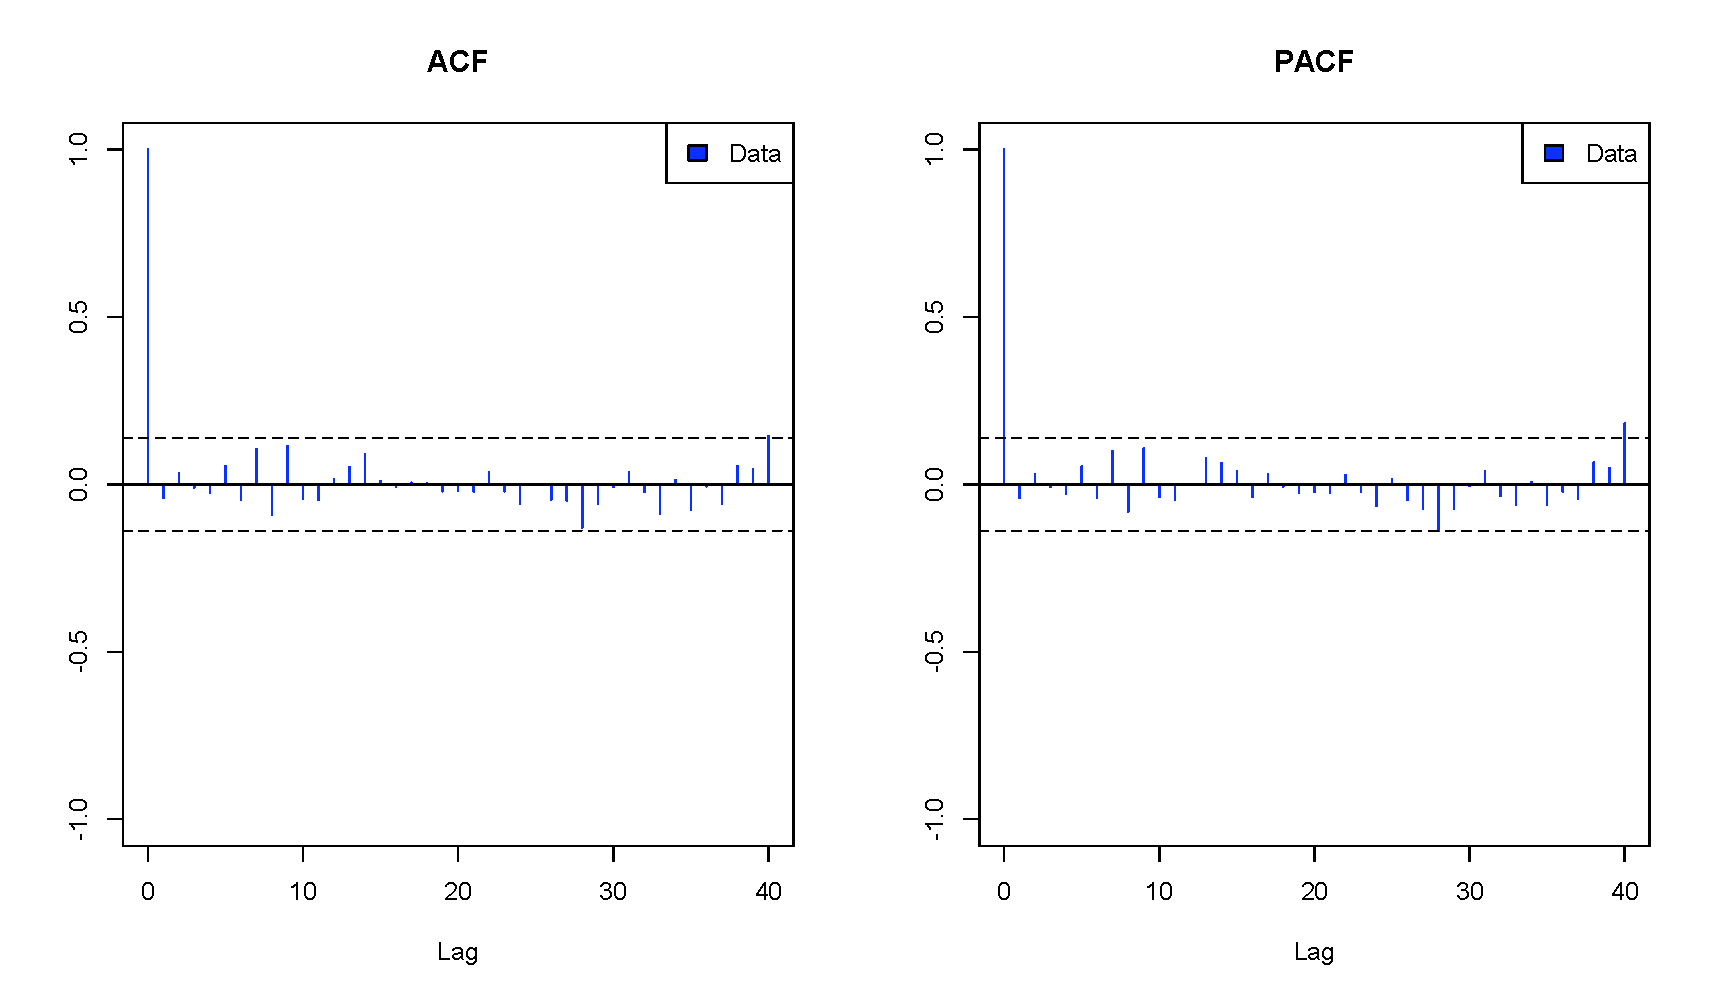
\includegraphics[scale=0.3]{Rplot-8.pdf}
\end{center}

\subsection{\tt plotc}
Plots one or two time series in color.
\begin{flalign*}
\text{\tt plotc(y1,y2=NULL)}\quad\left\{\begin{array}{ll}
{\tt y1} & \text{Blue line with knots}\\
{\tt y2} & \text{Red line without knots}
\end{array}\right.&&
\end{flalign*}

Example:
\begin{verbatim}
R> plotc(uspop)
\end{verbatim}

\begin{center}
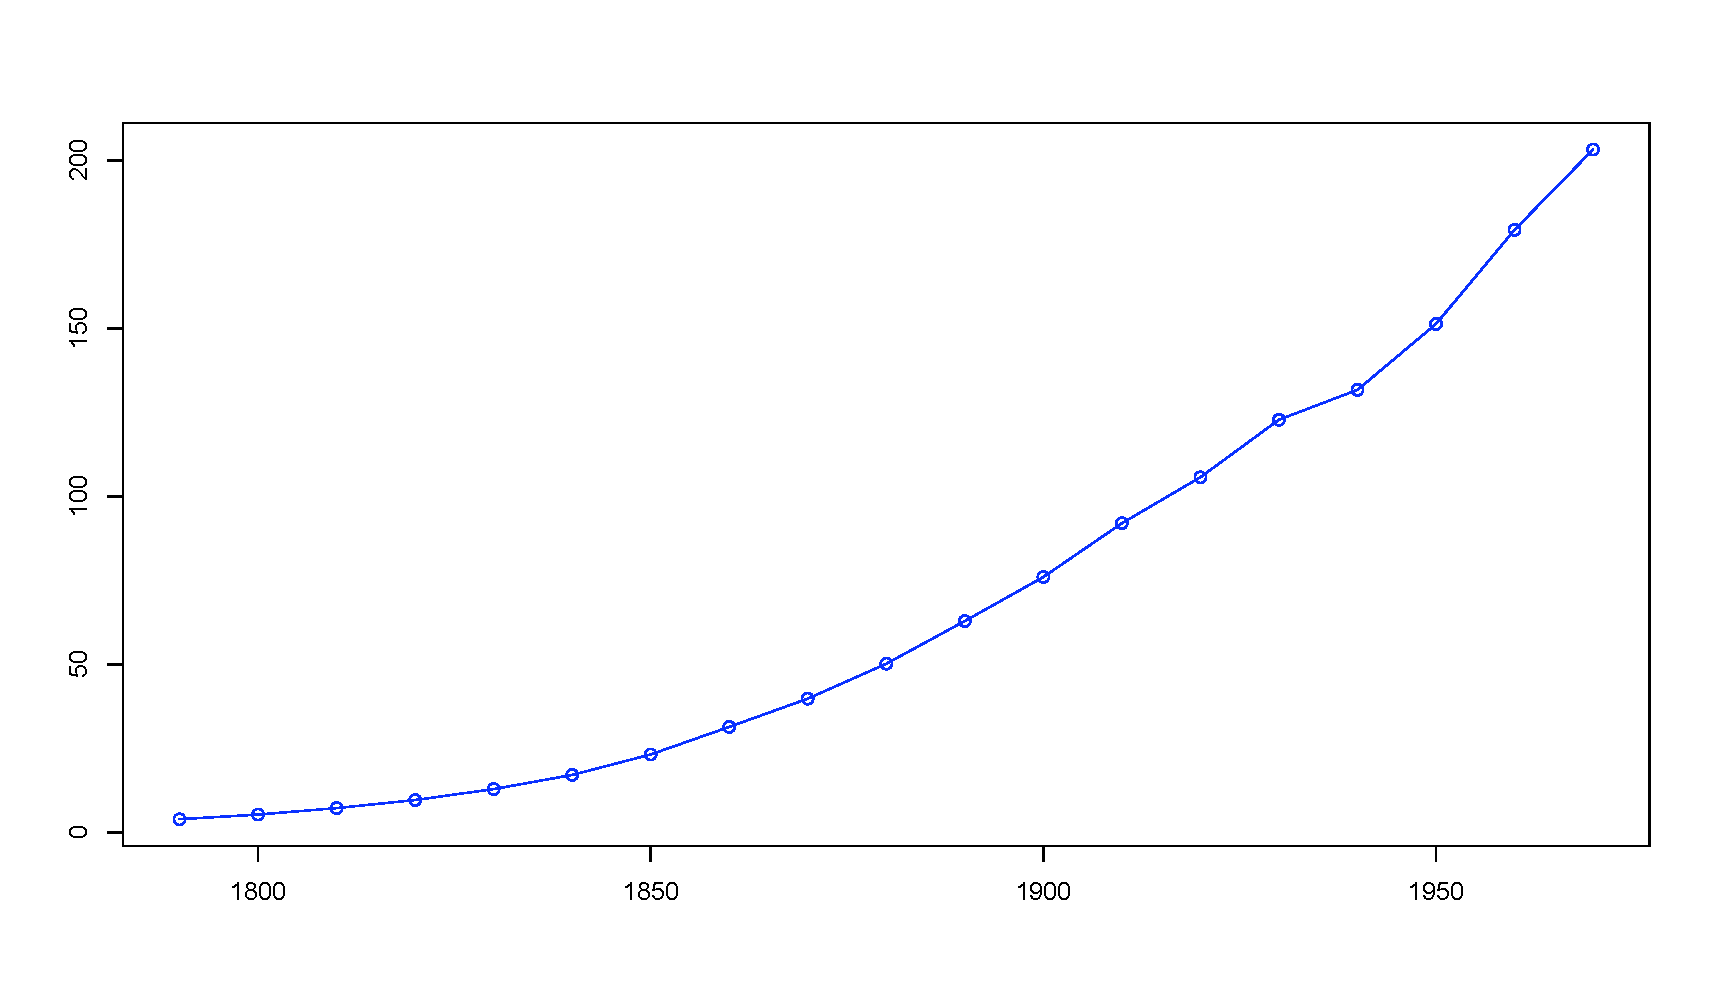
\includegraphics[scale=0.3]{Rplot-35.pdf}
\end{center}

\begin{verbatim}
R> y = trend(uspop,2)
R> plotc(uspop,y)
\end{verbatim}

\begin{center}
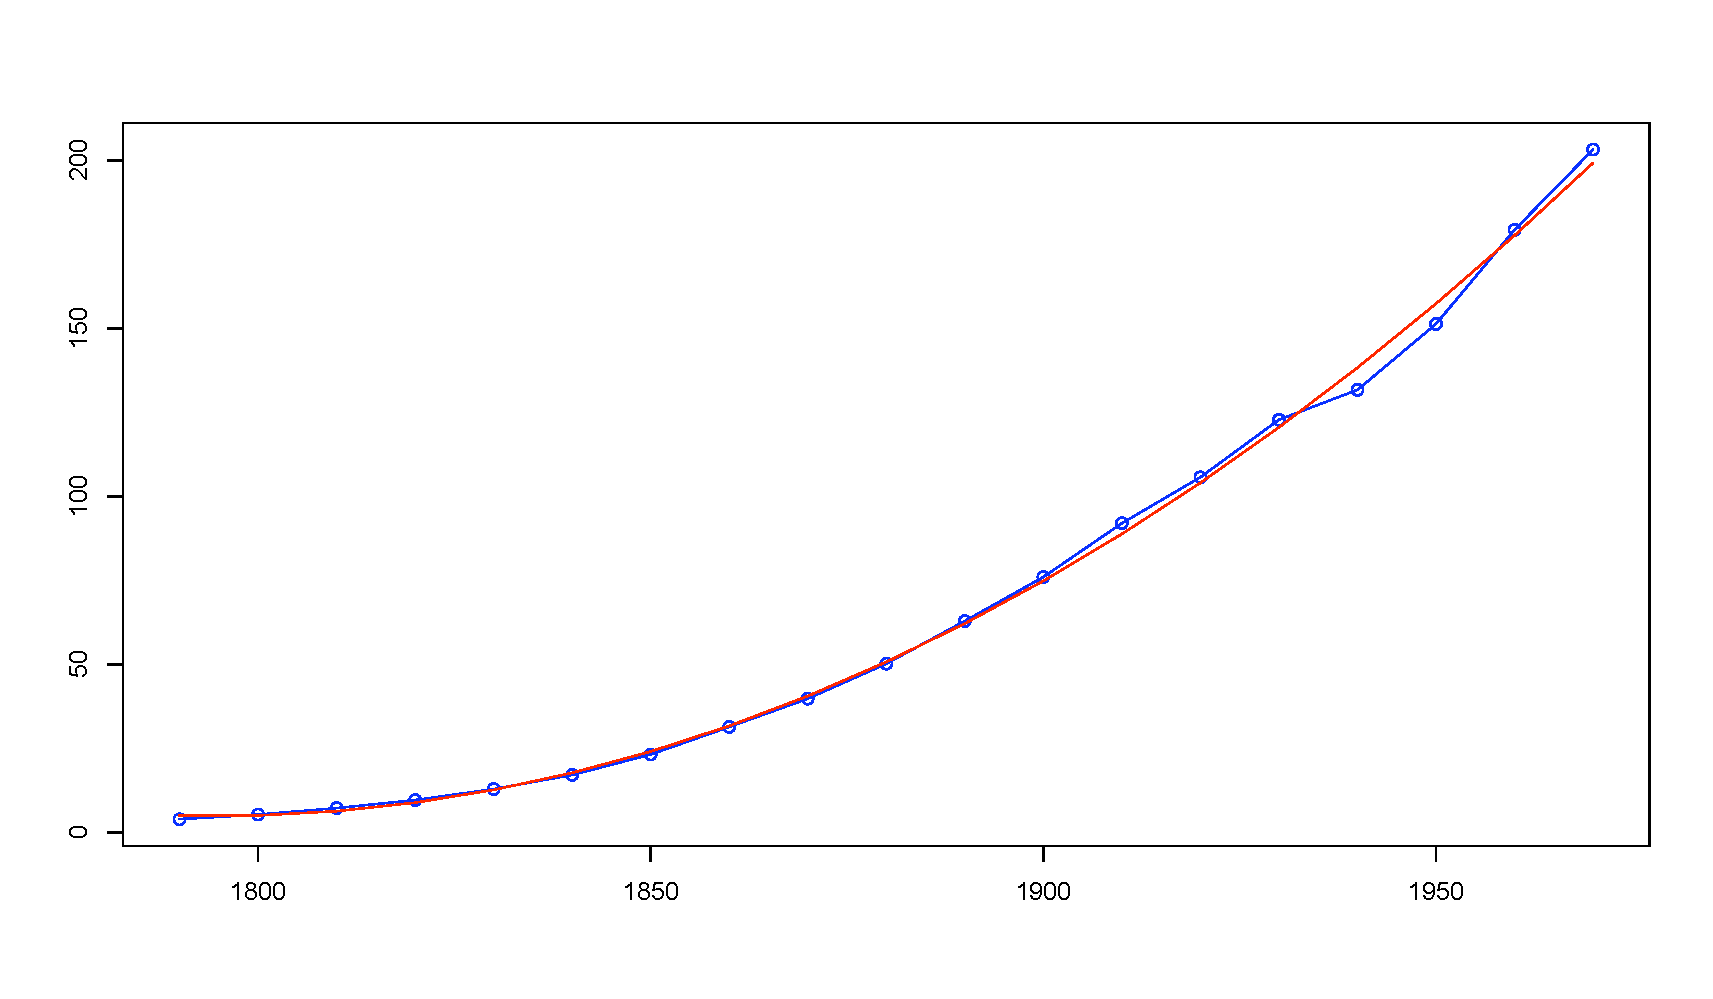
\includegraphics[scale=0.3]{Rplot-36.pdf}
\end{center}

\subsection{\tt plots}
Plots the spectrum of data or an ARMA model.
\begin{flalign*}
\text{\tt plots(u)}\quad\left\{\begin{array}{ll}
{\tt u} & \text{Time series data or ARMA model}
\end{array}\right.&&
\end{flalign*}

Example:

\begin{verbatim}
R> a = specify(ar=c(0,0,0.99))
R> plots(a)
\end{verbatim}

\begin{center}
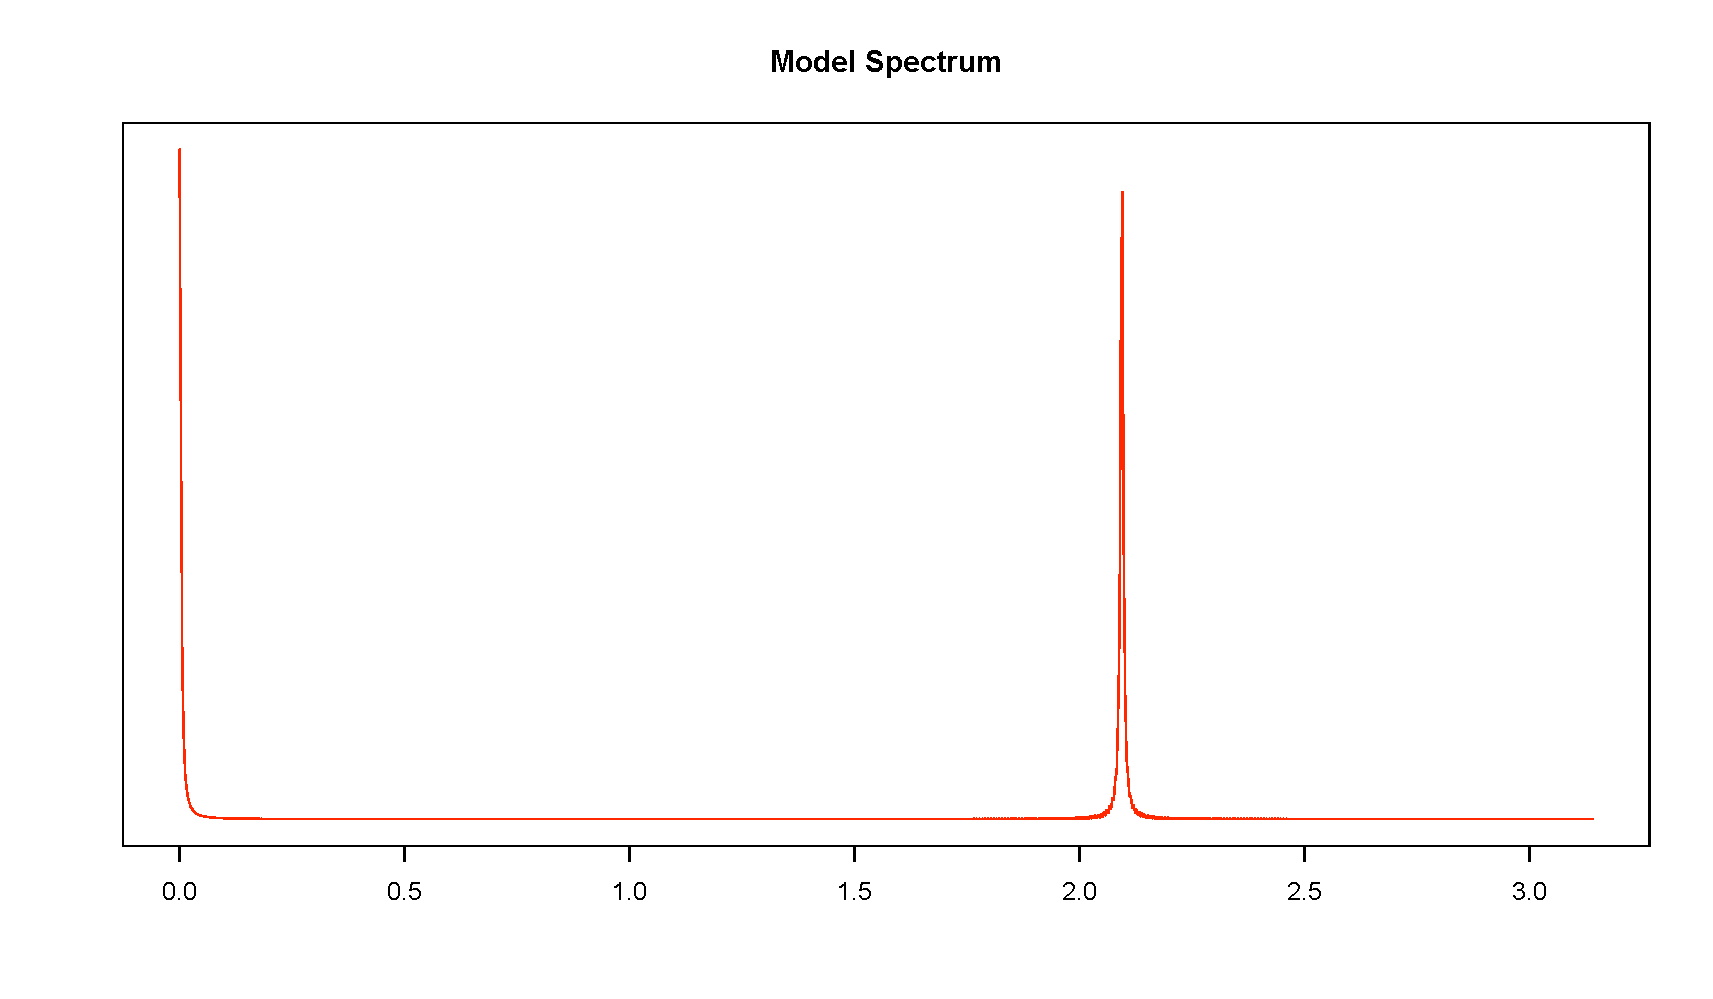
\includegraphics[scale=0.3]{Rplot-23.pdf}
\end{center}

\subsection{\tt Resid}
Returns the residuals of a time series model.
\begin{flalign*}
\text{\tt Resid(x,M=NULL,a=NULL)}\quad\left\{\begin{array}{ll}
{\tt x} & \text{Time series data}\\
{\tt M} & \text{Data model}\\
{\tt a} & \text{ARMA model}
\end{array}\right.&&
\end{flalign*}

Either {\tt M} or {\tt a} can be {\tt NULL} for none.
See below for details about the data model.
The returned residuals always have zero mean.

\bigskip
In the following example, {\tt Resid} and {\tt test}
are used
to check for stationarity of the transformed
data.
Then they are used again to check that the overall
model reduces the data to white noise.

\begin{verbatim}
R> M = c("log","season",12,"trend",1)
R> e = Resid(airpass,M)
R> test(e)
R> a = arma(e,1,0)
R> ee = Resid(airpass,M,a)
R> test(ee)
\end{verbatim}

The data model {\tt M} is a vector of function names.
The functions are applied to the data in left to right order.
There are five functions from which to choose.

\begin{quote}
\begin{tabular}{ll}
{\tt diff} & Difference the data\\
{\tt hr} & Subtract harmonic components\\
{\tt log} & Take the log of the data\\
{\tt season} & Subtract seasonal component\\
{\tt trend} & Subtract trend component\\
\end{tabular}
\end{quote}

A function name may be followed by one or more arguments.

\bigskip
{\tt diff} has a single argument, the lag.

\bigskip
{\tt hr} has one or more arguments, each specifying the number
of observations per harmonic period.

\bigskip
{\tt log} has no arguments.

\bigskip
{\tt season} has one argument, the number of observations per season.

\bigskip
{\tt trend} has one argument, the polynomial order of the trend,
(1 for linear, 2 for quadratic, etc.)

\bigskip
A data model is built up by concatenating the function
names and arguments. For example, the following vector takes the
log of the data, then subtracts a seasonal component of period twelve
then subtracts a linear trend component.

\begin{verbatim}
R> M = c("log","season",12,"trend",1)
\end{verbatim}

At the end of the data model there
is an implied subtraction of the mean operation.
Hence the resulting time series always has zero mean.

\subsection{\tt season}
Returns the seasonal component of time series data.
\begin{flalign*}
\text{\tt season(x,d)}\quad\left\{\begin{array}{ll}
{\tt x} & \text{Time series data}\\
{\tt d} & \text{Number of observations per season}
\end{array}\right.&&
\end{flalign*}

Example:

\begin{verbatim}
R> s = season(deaths,12)
R> plotc(deaths,s)
\end{verbatim}

\begin{center}
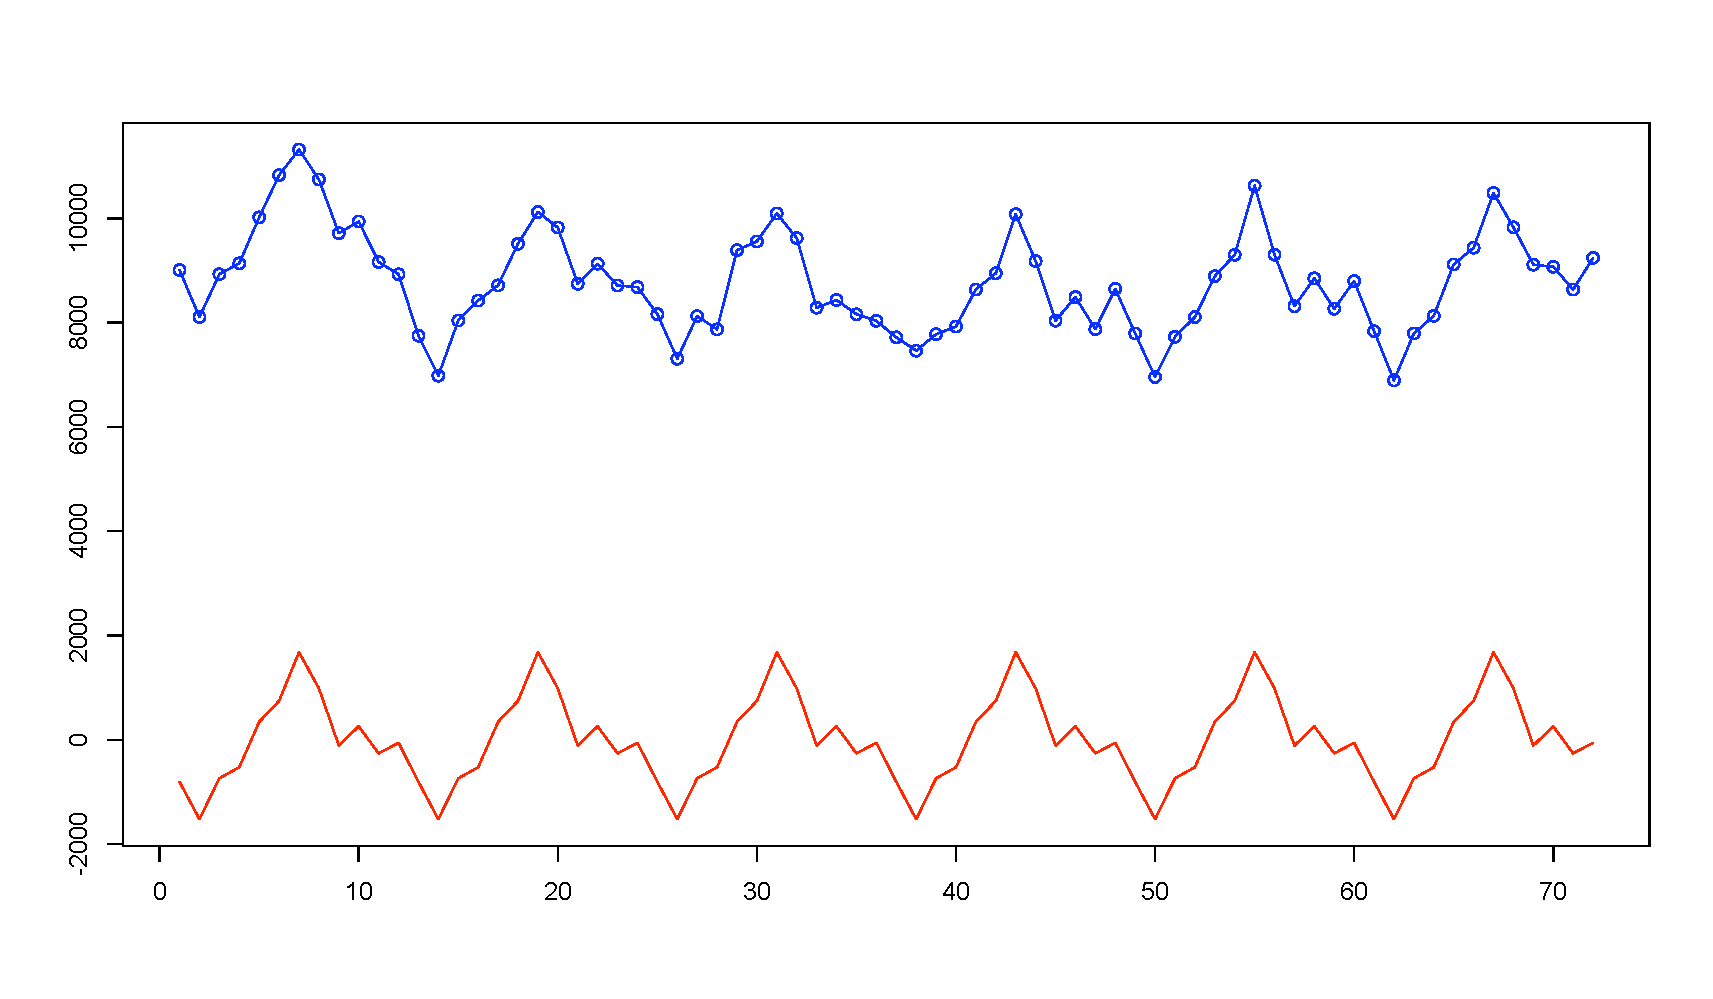
\includegraphics[scale=0.3]{Rplot-1.pdf}
\end{center}

\subsection{\tt sim}
Generate synthetic observations for an ARMA model.
\begin{flalign*}
\text{\tt sim(a,n)}\quad\left\{\begin{array}{ll}
{\tt a} & \text{ARMA model}\\
{\tt n} & \text{Number of synthetic observations required}
\end{array}\right.&&
\end{flalign*}

The ARMA model is a list with the following components.

\begin{quote}
\begin{tabular}{ll}
{\tt \$phi} & AR coefficients $\phi_1$, $\ldots\,$, $\phi_p$\\
{\tt \$theta} & MA coefficients $\theta_1$, $\ldots\,$, $\theta_q$\\
{\tt \$sigma2} & White noise variance $\sigma^2$
\end{tabular}
\end{quote}

Example:
\begin{verbatim}
R> a = specify(ar=c(0,0,0.99))
R> x = sim(a,60)
R> plotc(x)
\end{verbatim}

\begin{center}
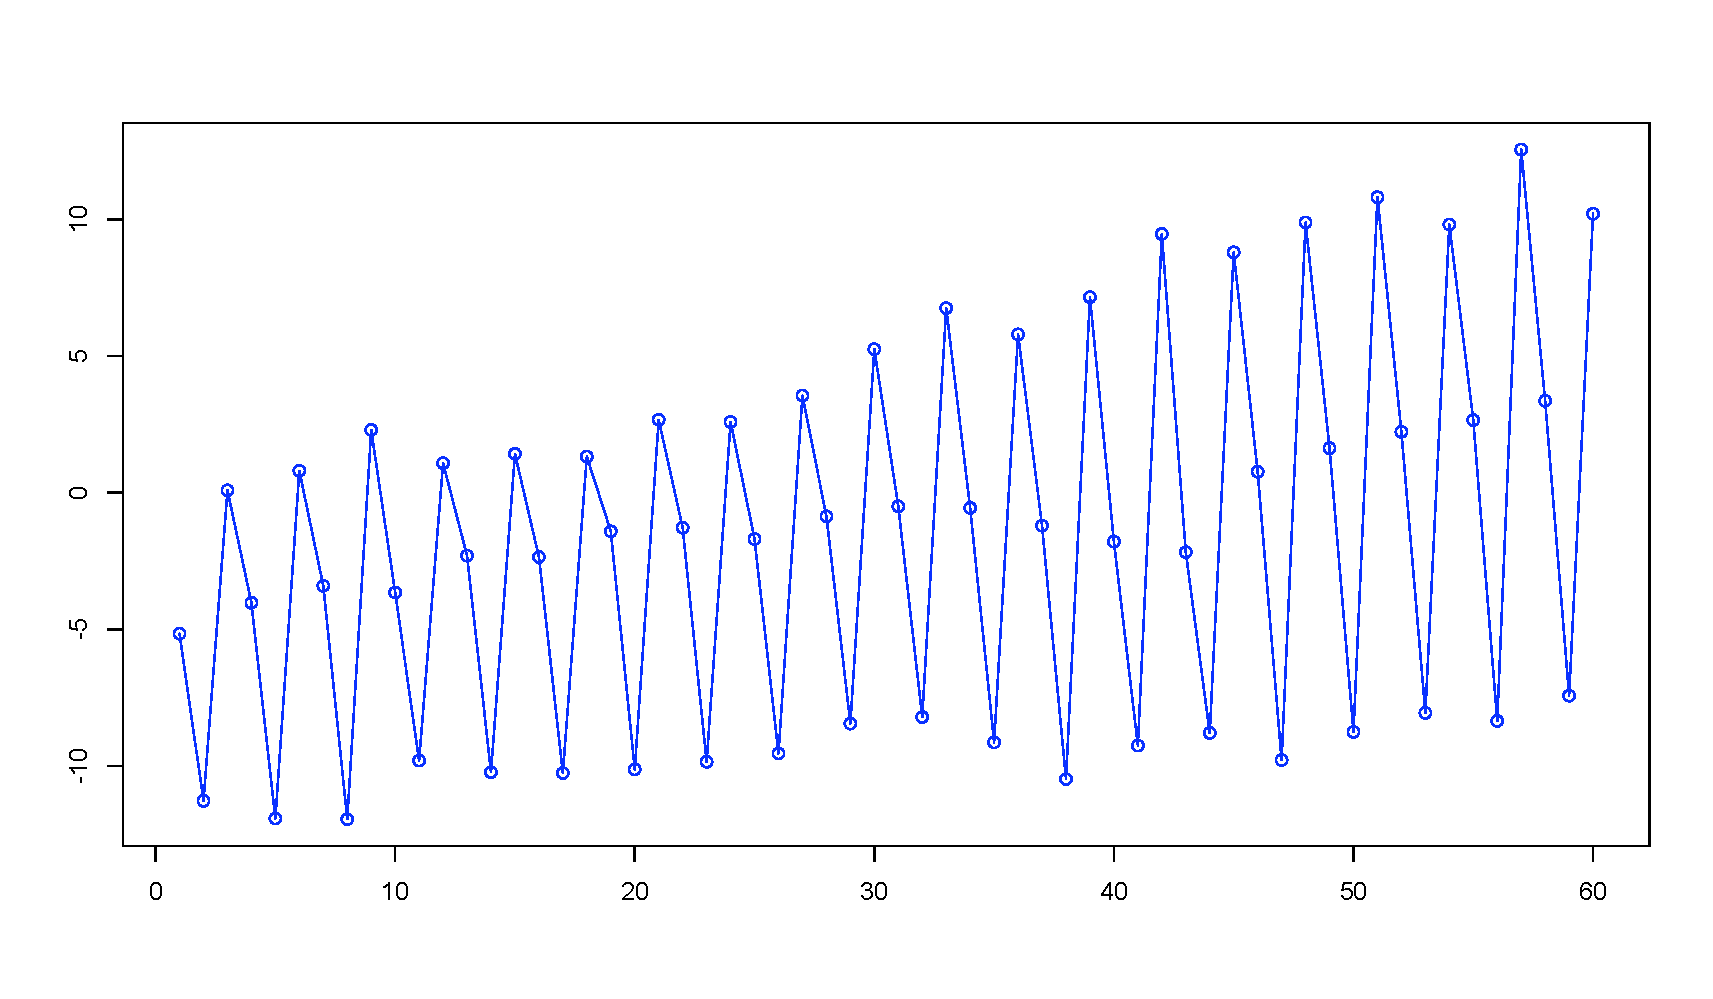
\includegraphics[scale=0.3]{Rplot-24.pdf}
\end{center}

\subsection{\tt smooth.exp}
Applies an exponential smoothing filter to data and returns the result.
\begin{flalign*}
\text{\tt smooth.exp(x,a)}\quad\left\{\begin{array}{ll}
{\tt x} & \text{Time series data}\\
{\tt a} & \text{0 to 1, zero is maximum smoothness.}
\end{array}\right.&&
\end{flalign*}

Example:

\begin{verbatim}
R> y = smooth.exp(strikes,0.4)
R> plotc(strikes,y)
\end{verbatim}

\begin{center}
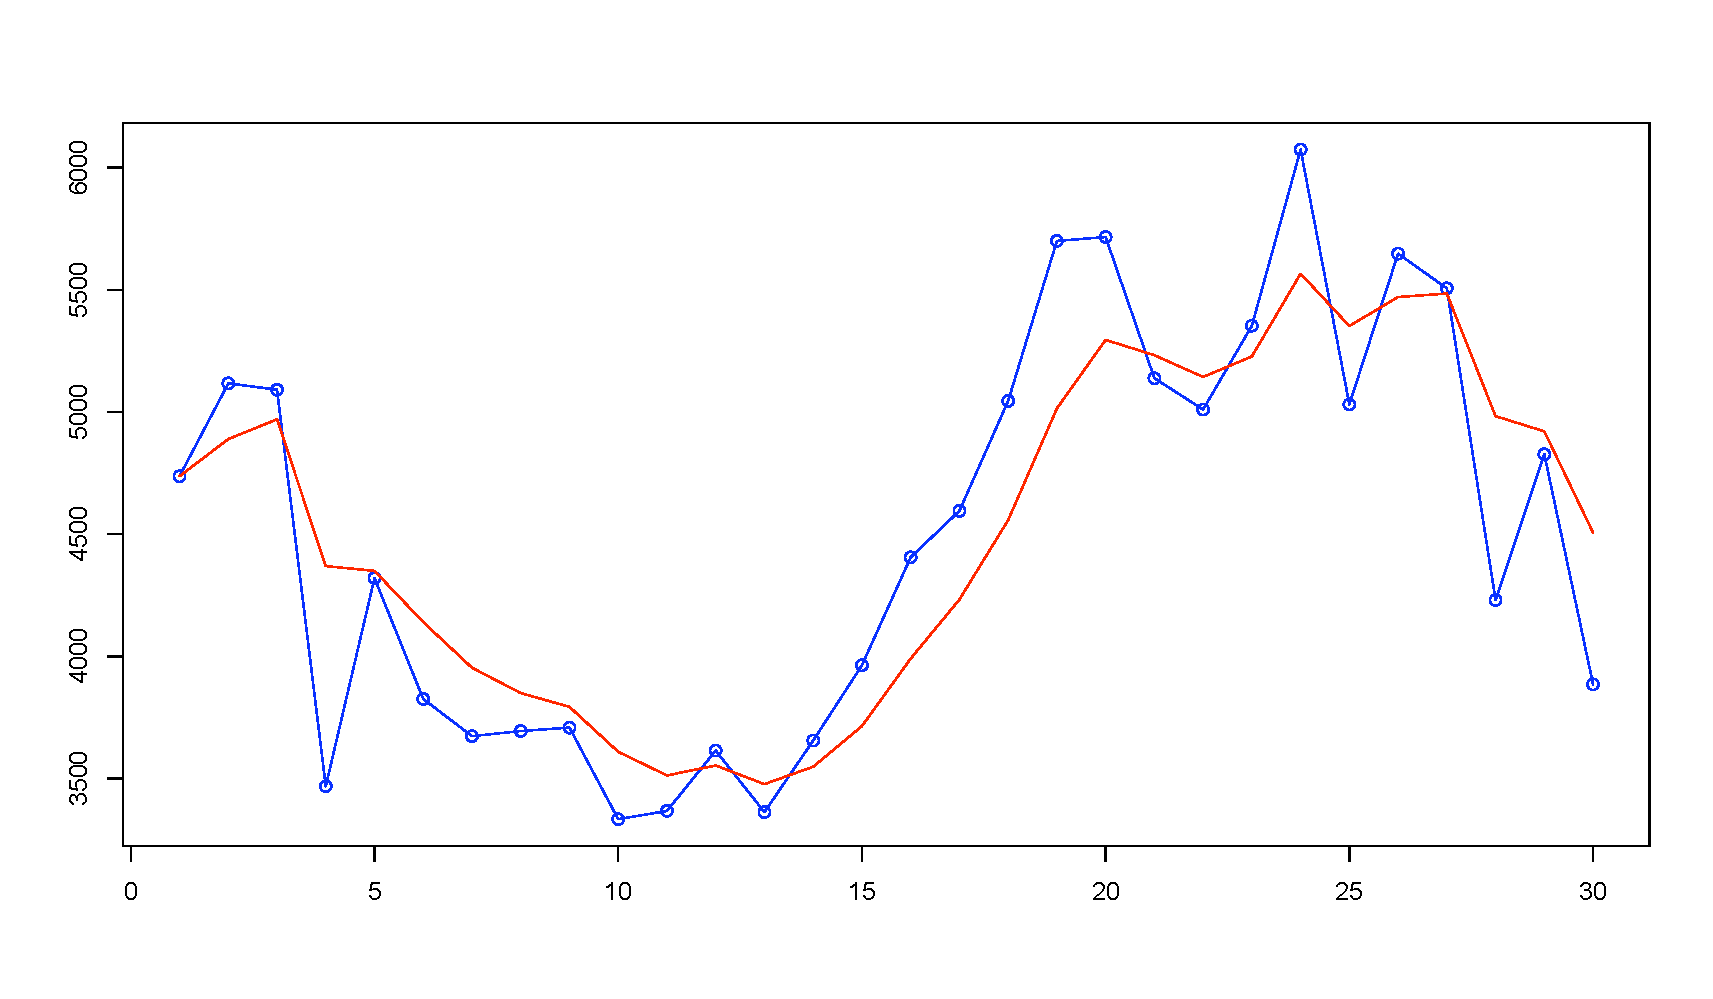
\includegraphics[scale=0.3]{Rplot-11.pdf}
\end{center}

\subsection{\tt smooth.fft}
Applies a low pass filter to data and returns the result.
\begin{flalign*}
\text{\tt smooth.fft(x,c)}\quad\left\{\begin{array}{ll}
{\tt x} & \text{Time series data}\\
{\tt c} & \text{Cut-off freq. 0--1}
\end{array}\right.&&
\end{flalign*}

The cut-off frequency is specified as a fraction.
For example, ${\tt c}=0.25$ passes the lowest 25\% of the frequency spectrum.

\bigskip
Example:

\begin{verbatim}
R> y = smooth.fft(signal,0.035)
R> plotc(signal,y)
\end{verbatim}

\begin{center}
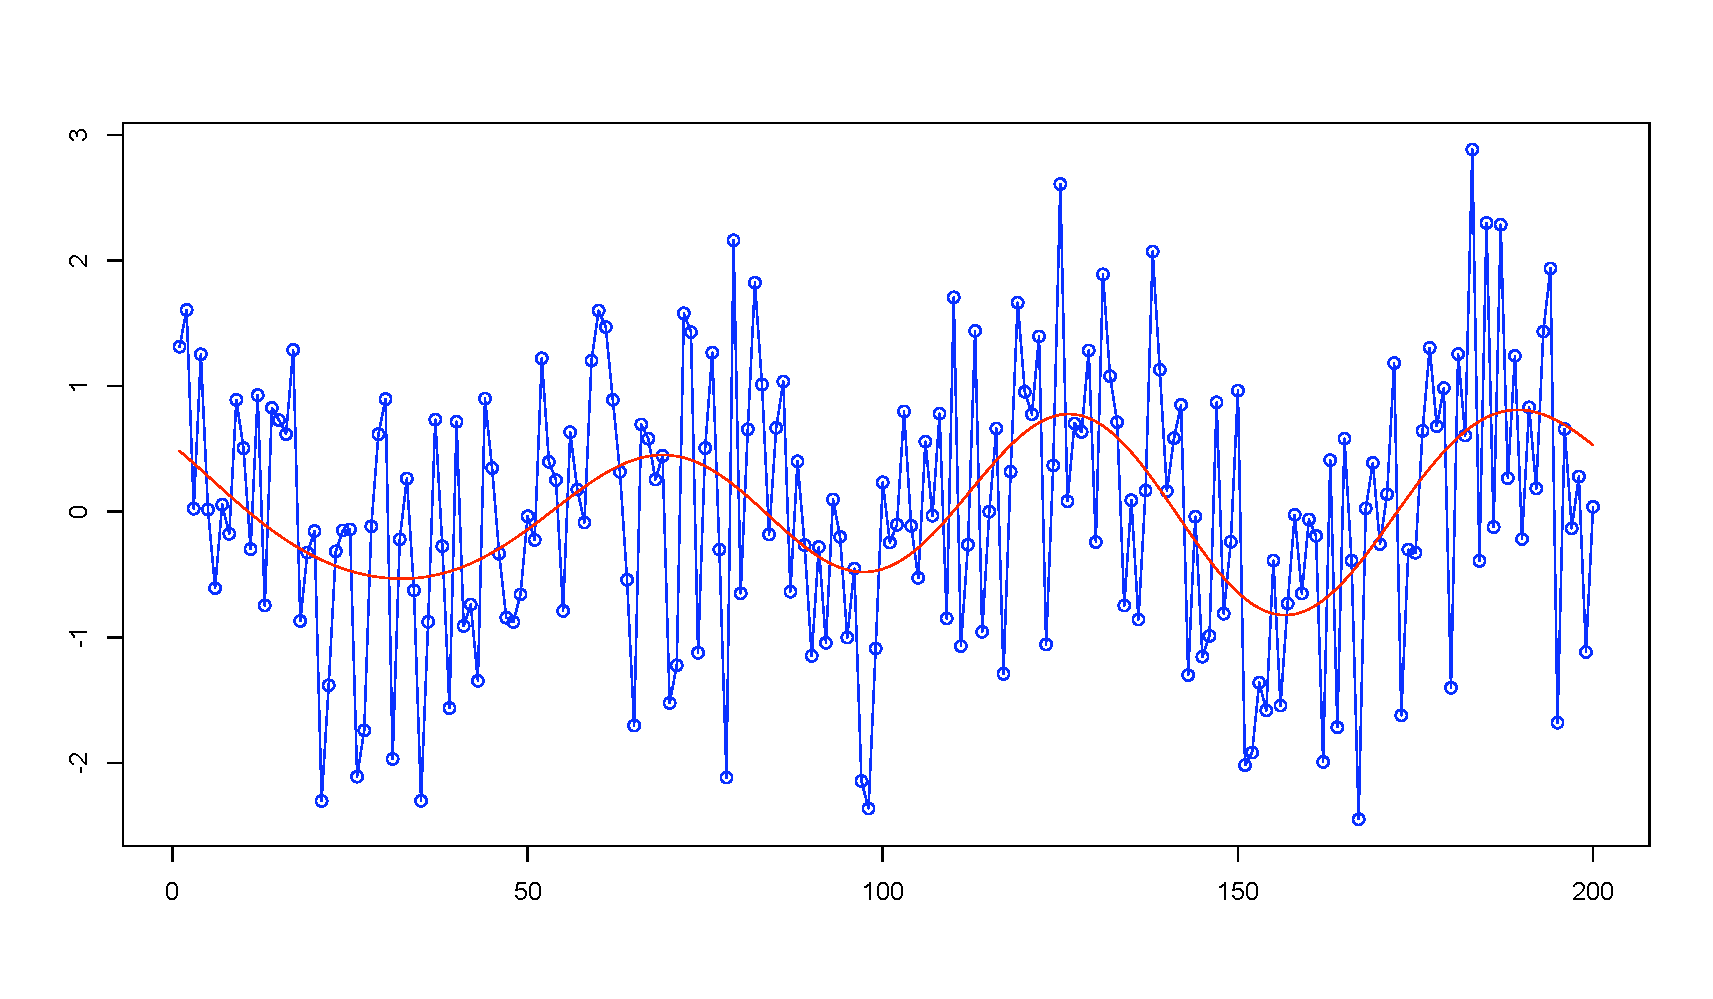
\includegraphics[scale=0.3]{Rplot-2.pdf}
\end{center}

\subsection{\tt smooth.ma}
Applies a moving average filter to data and returns the result.
\begin{flalign*}
\text{\tt smooth.ma(x,q)}\quad\left\{\begin{array}{ll}
{\tt x} & \text{Time series data}\\
{\tt q} & \text{Filter order}
\end{array}\right.&&
\end{flalign*}

Example:

\begin{verbatim}
R> y = smooth.ma(strikes,2)
R> plotc(strikes,y)
\end{verbatim}

\begin{center}
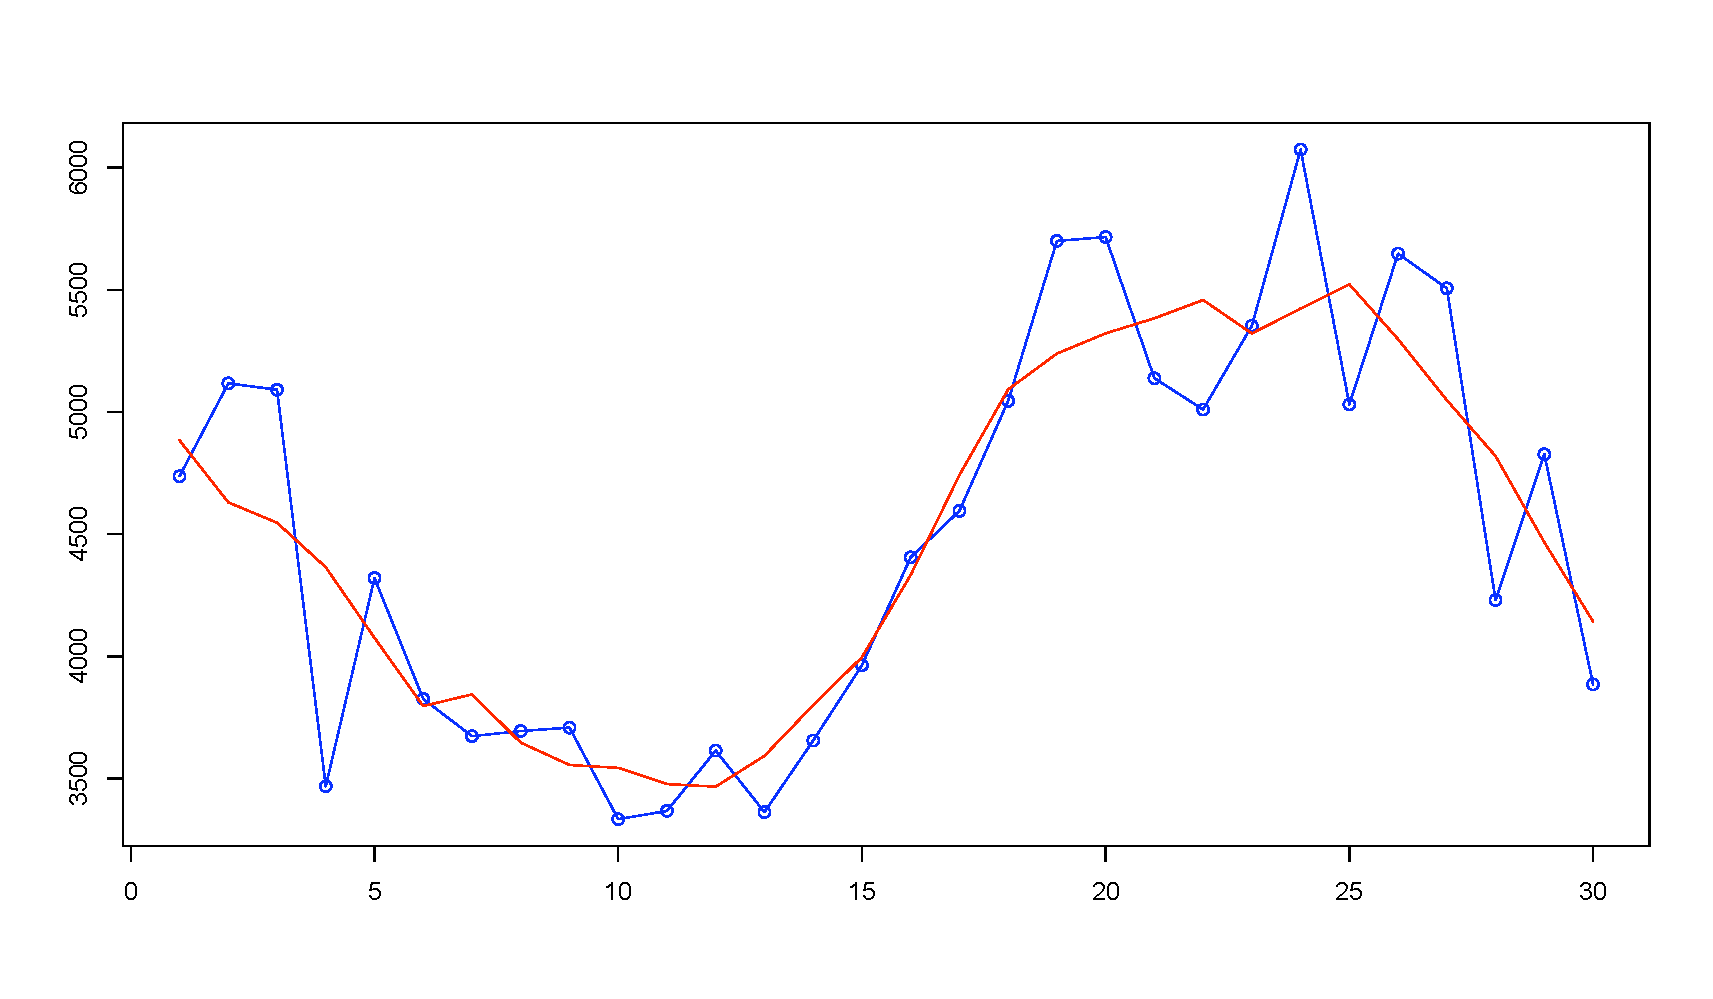
\includegraphics[scale=0.3]{Rplot-10.pdf}
\end{center}

\bigskip
From page 25 of {\it Introduction to Time Series and Forecasting},
\[
Y_t=\frac{1}{2q+1}\sum_{j=-q}^qX_{t-j}
\]
Hence for $q=2$ the moving average filter is
\[
Y_t=\frac{1}{5}(X_{t-2}+X_{t-1}+X_t+X_{t+1}+X_{t+2})
\]

\subsection{\tt smooth.rank}
Passes the mean and the $k$ frequencies
with the highest amplitude.
The remainder of the spectrum is filtered out.
\begin{flalign*}
\text{\tt smooth.rank(x,k)}\quad\left\{
\begin{array}{ll}
{\tt x} & \text{Time series data}\\
{\tt k} & \text{Rank}
\end{array}\right.&&
\end{flalign*}

Example:

\begin{verbatim}
R> y = smooth.rank(deaths,1)
R> plot(deaths,y)
\end{verbatim}

\begin{center}
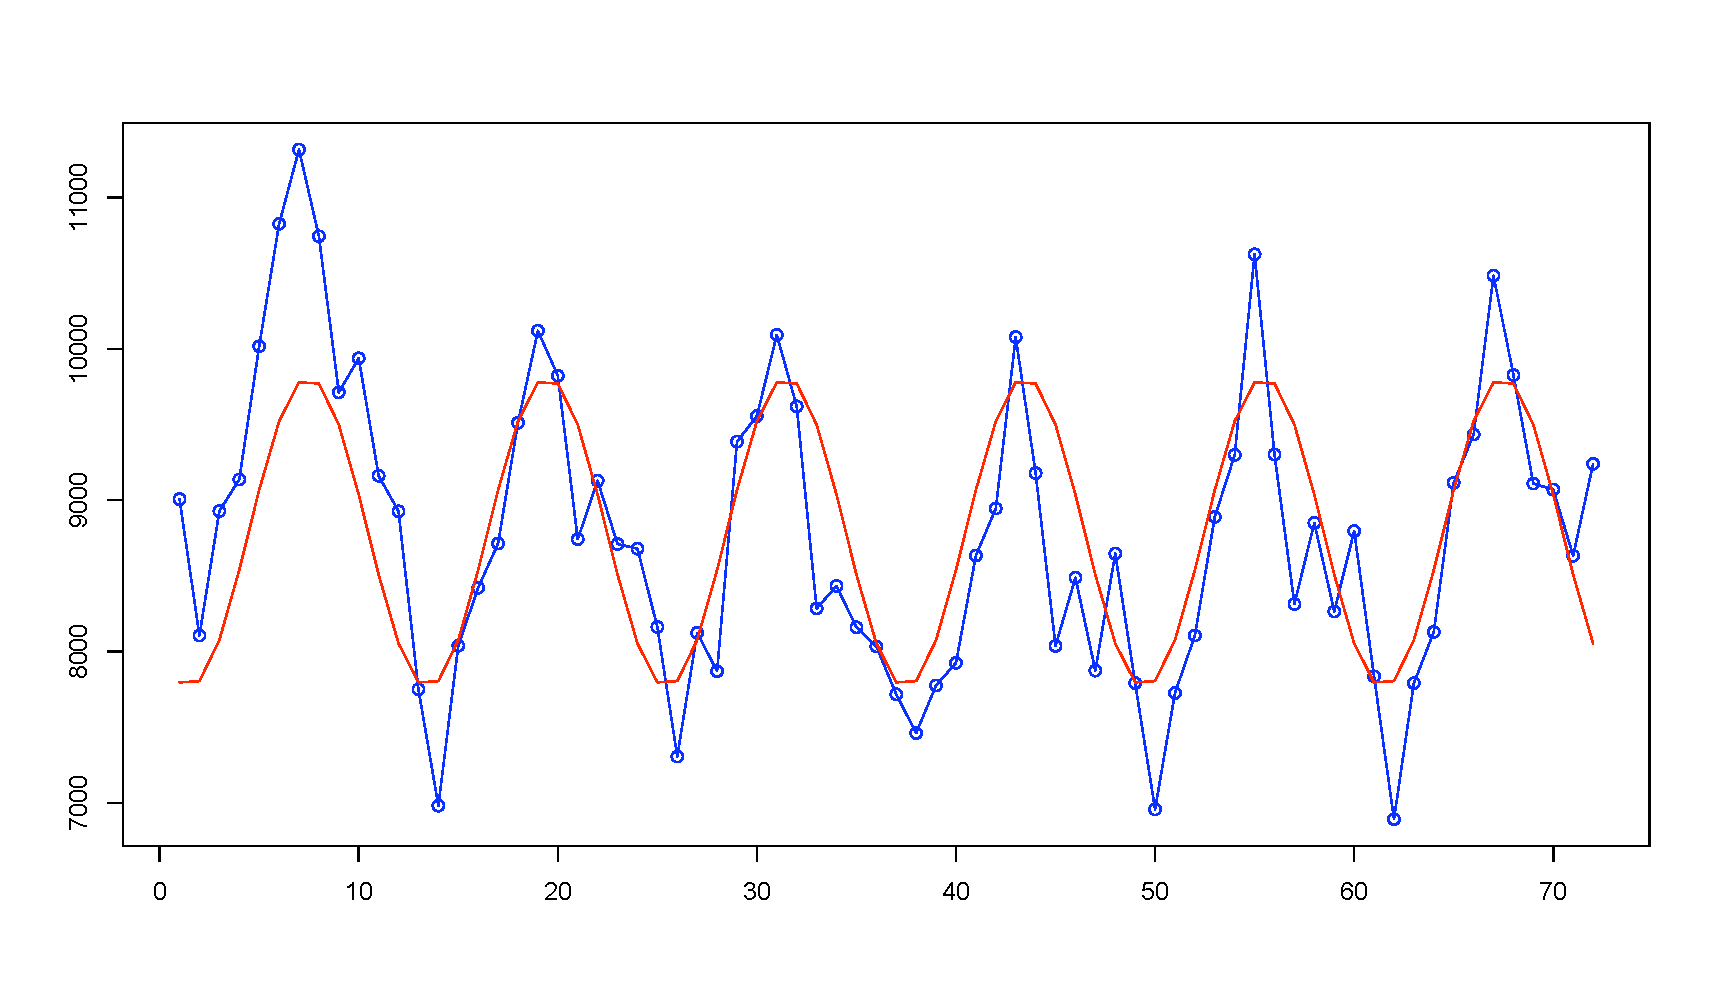
\includegraphics[scale=0.3]{Rplot-14.pdf}
\end{center}

\begin{verbatim}
R> y = smooth.rank(deaths,2)
R> plot(deaths,y)
\end{verbatim}

\begin{center}
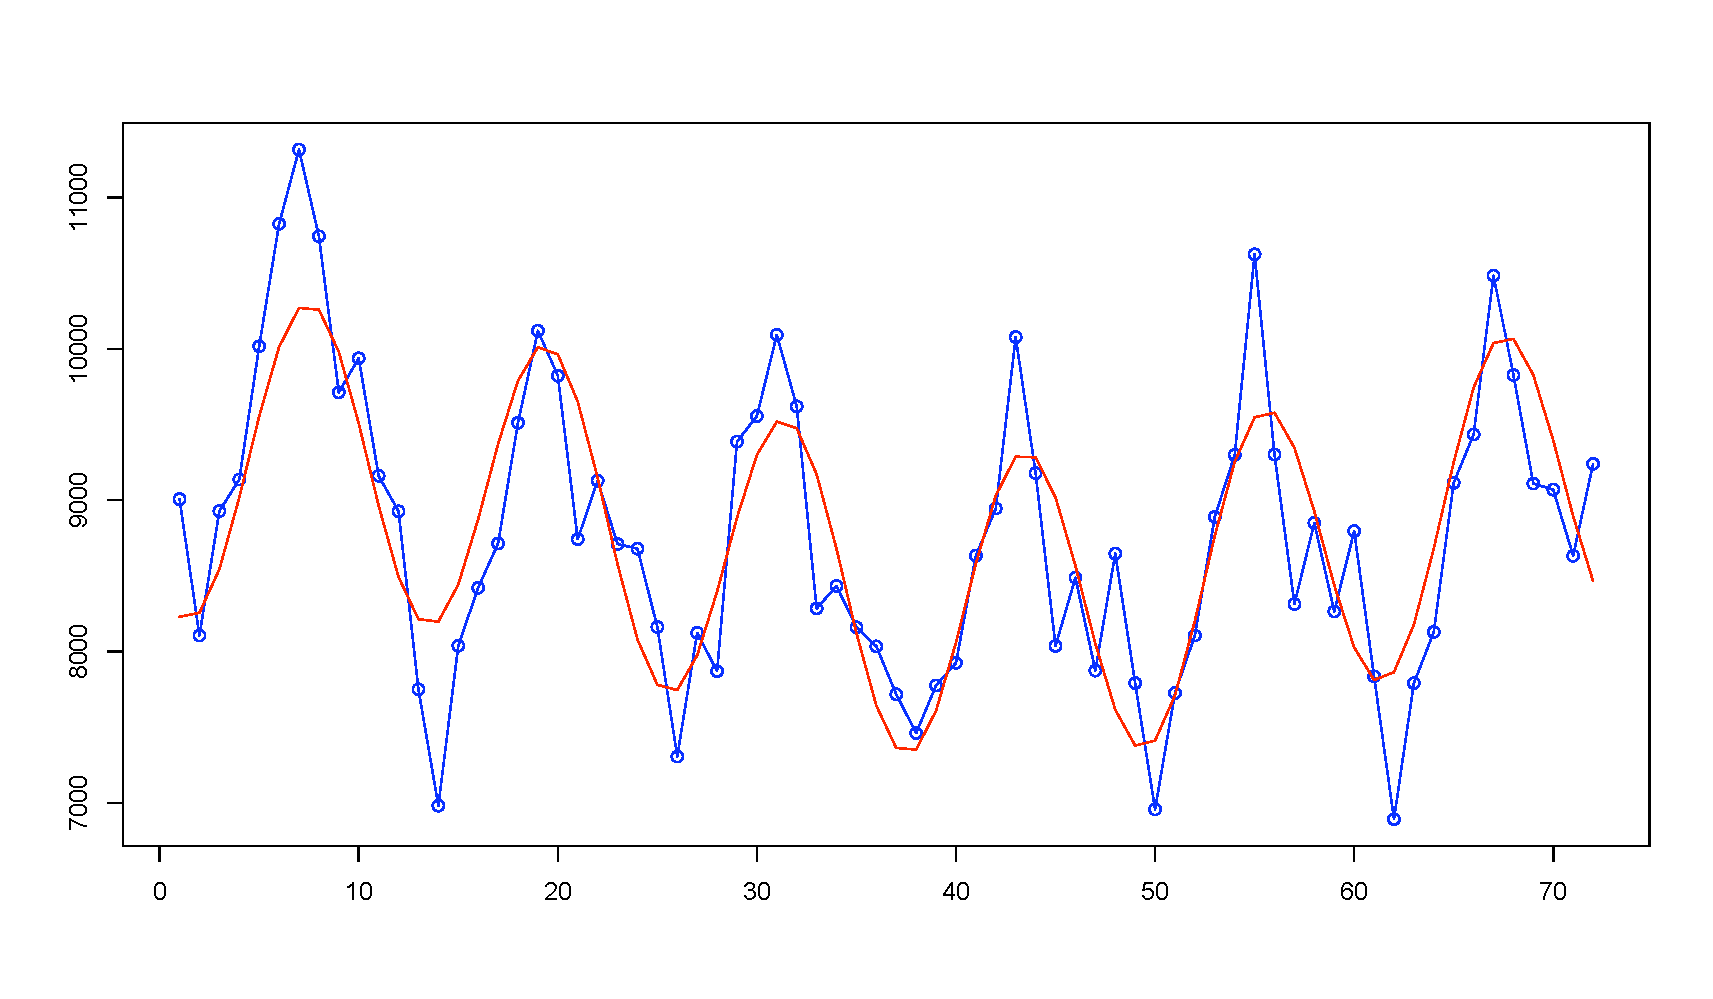
\includegraphics[scale=0.3]{Rplot-15.pdf}
\end{center}

\subsection{\tt specify}
Returns an ARMA model with the specified parameters.
\begin{flalign*}
\text{\tt specify(ar=0,ma=0,sigma2=1)}\quad\left\{\begin{array}{ll}
{\tt ar} & \text{AR coefficients \tt[1:p]}=\phi_1,\ldots,\phi_p\\
{\tt ma} & \text{MA coefficients \tt[1:q]}=\theta_1,\ldots,\theta_q\\
{\tt sigma2} & \text{White noise variance $\sigma^2$}
\end{array}\right.&&
\end{flalign*}

The signs of the coefficients correspond to the following model.
\[
X_t=\phi_1X_{t-1}+\phi_2X_{t-2}+\cdots+Z_t+\theta_1Z_{t-1}+\theta_2Z_{t-2}+\cdots
\]

Example:

\begin{verbatim}
R> specify(ar=c(0,0,0.99))
$phi
[1] 0.00 0.00 0.99

$theta
[1] 0

$sigma2
[1] 1
\end{verbatim}

\subsection{\tt test}
Test residuals for randomness.
\begin{flalign*}
\text{\tt test(e)}\quad\left\{\begin{array}{ll}
{\tt e} & \text{Residuals}
\end{array}\right.&&
\end{flalign*}

Example:

\begin{verbatim}
R> M = c("log","season",12,"trend",1)
R> e = Resid(airpass,M)
R> test(e)
Null hypothesis: Residuals are iid noise.
Test                        Distribution Statistic   p-value
Ljung-Box Q                Q ~ chisq(20)    412.43         0 *
McLeod-Li Q                Q ~ chisq(20)     41.29    0.0034 *
Turning points T     (T-94.7)/5 ~ N(0,1)        85    0.0545
Diff signs S       (S-71.5)/3.5 ~ N(0,1)        68     0.314
Rank P           (P-5148)/289.5 ~ N(0,1)      5187    0.8928
\end{verbatim}

\begin{center}
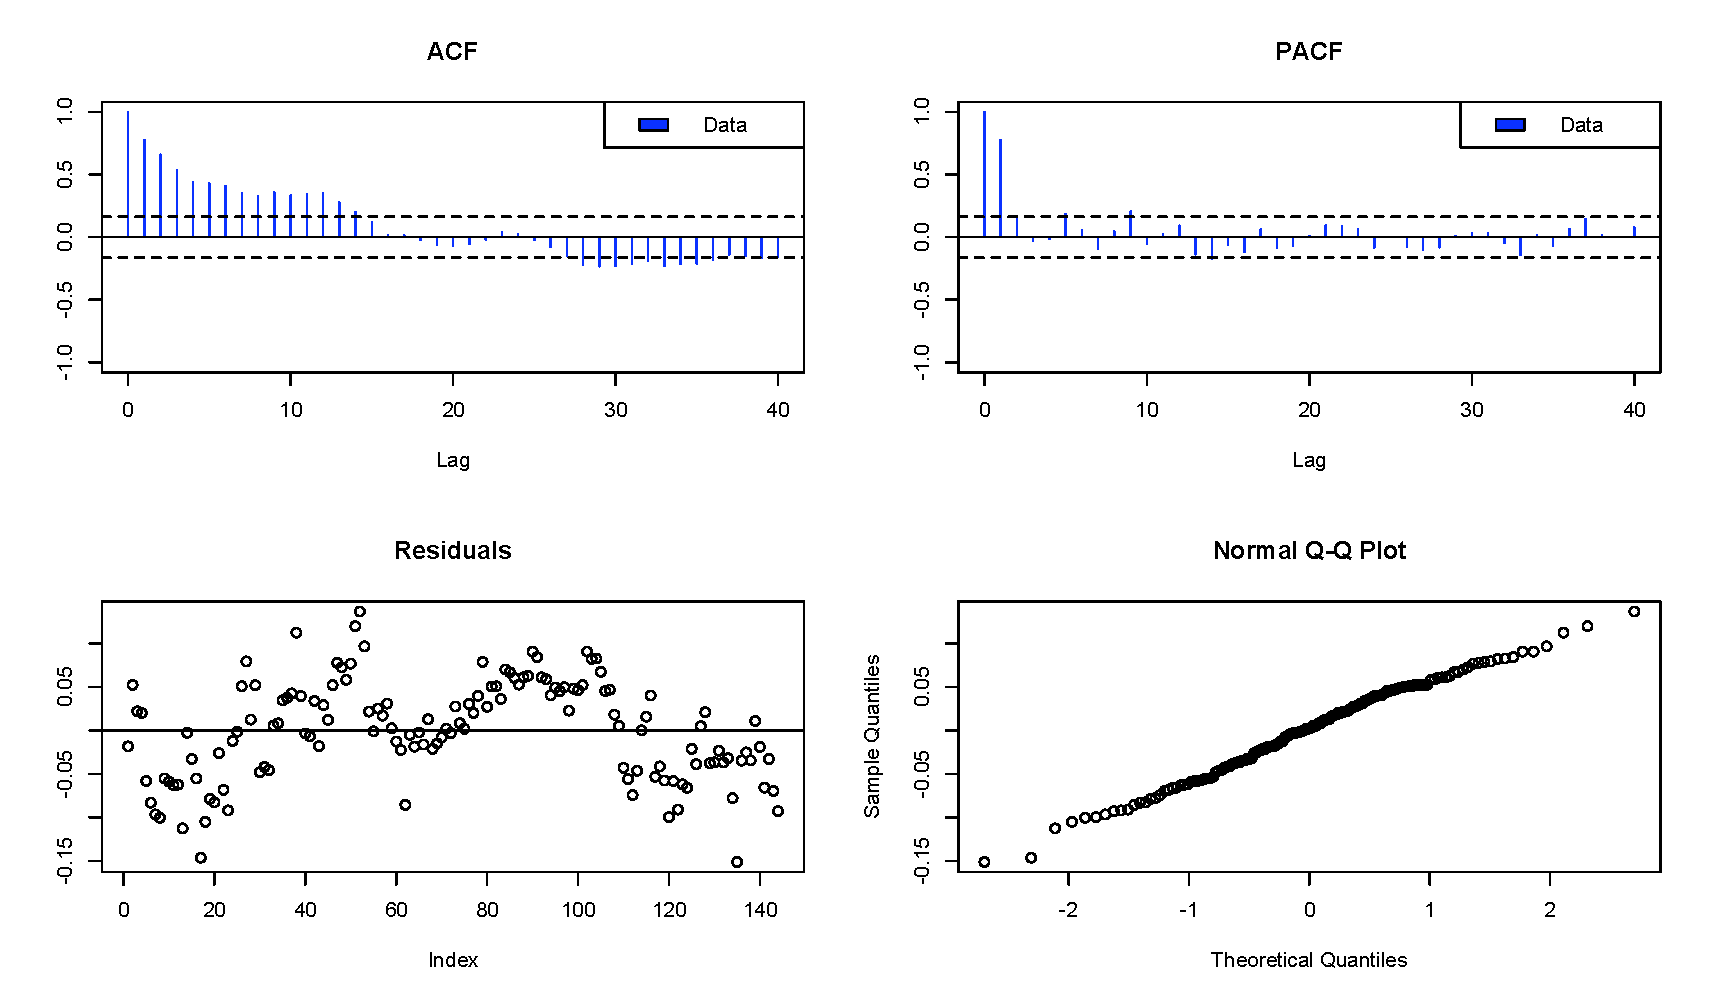
\includegraphics[scale=0.4]{Rplot-33.pdf}
\end{center}

\subsection{\tt trend}
Returns the trend component of time series data.
\begin{flalign*}
\text{\tt trend(x,p)}\quad\left\{\begin{array}{ll}
{\tt x} & \text{Time series data}\\
{\tt n} & \text{Polynomial order}\\
\end{array}\right.&&
\end{flalign*}

Example:
\begin{verbatim}
R> y = trend(uspop,2)
R> plotc(uspop,y)
\end{verbatim}

\begin{center}
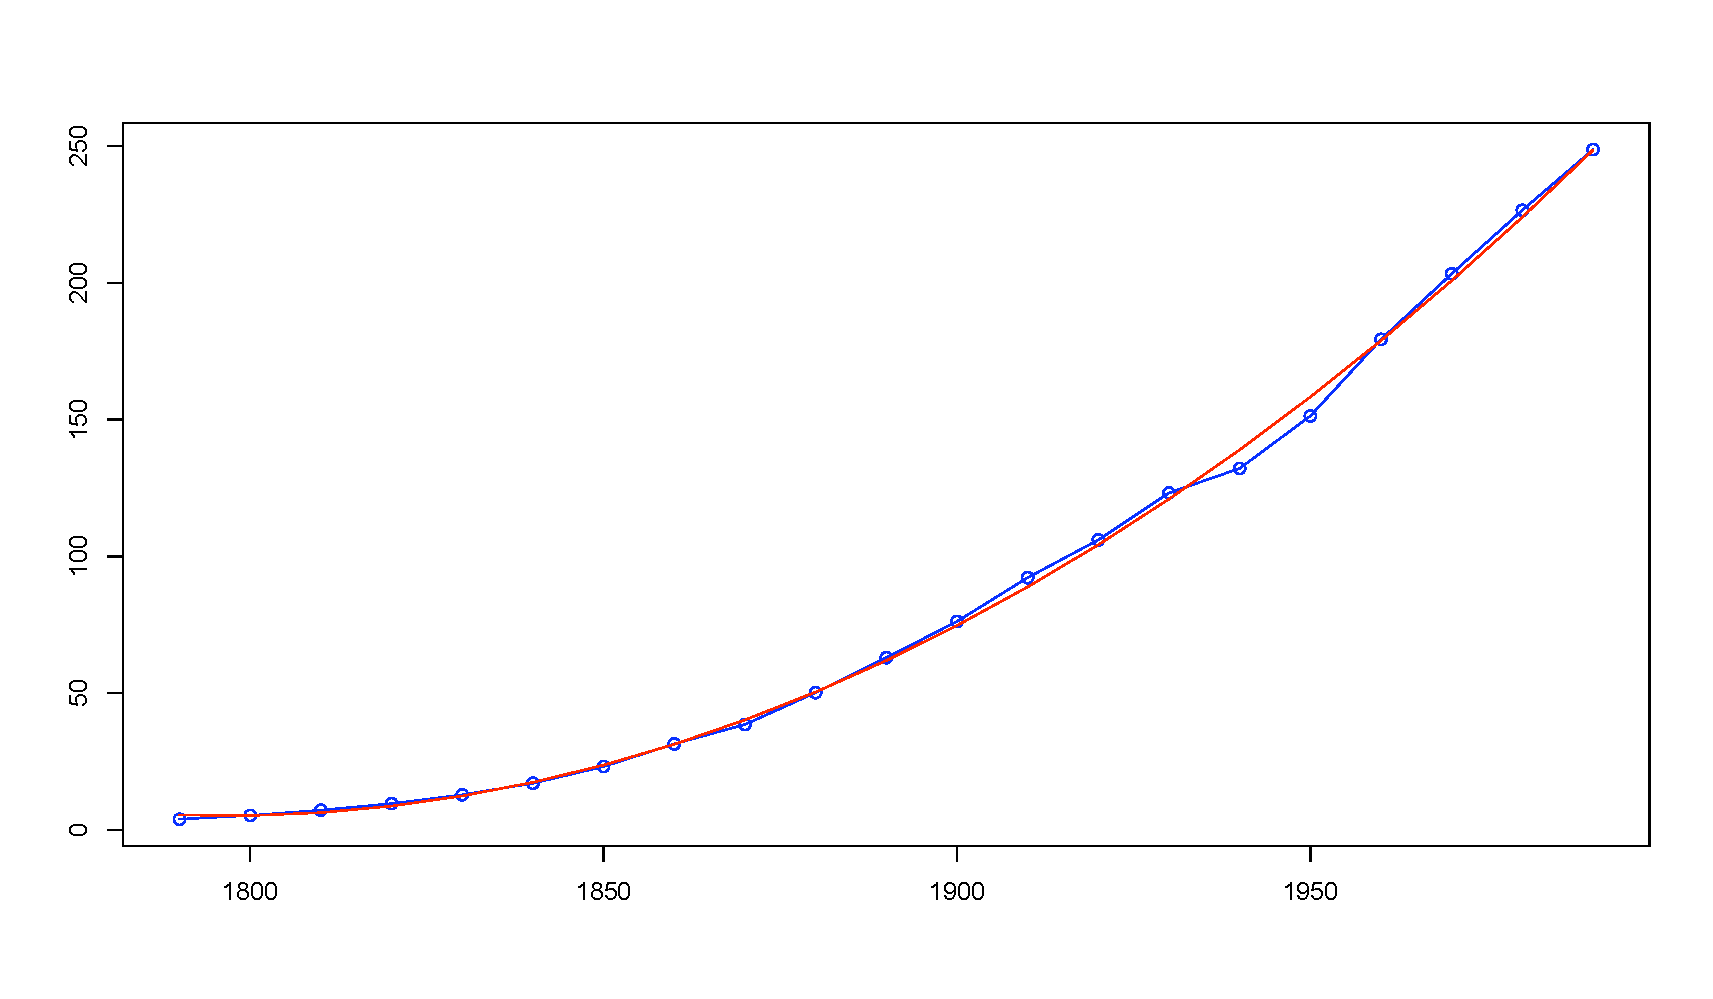
\includegraphics[scale=0.3]{Rplot-3.pdf}
\end{center}

\subsection{\tt yw}
Estimates AR coefficients using the Yule-Walker method.
\begin{flalign*}
\text{\tt yw(x,p)}\quad\left\{\begin{array}{ll}
{\tt x} & \text{Time series data}\\
{\tt p} & \text{AR order}
\end{array}\right.&&
\end{flalign*}

Returns an ARMA model with the following components.

\begin{quote}
\begin{tabular}{ll}
{\tt \$phi} & AR coefficients $\text{\tt[1:p]}=\phi_1,\ldots,\phi_p$\\
{\tt \$theta} & 0\\
{\tt \$sigma2} & White noise variance $\sigma^2$\\
{\tt \$aicc} & Akaike information criterion corrected\\
{\tt \$se.phi} & Standard errors for AR coefficients\\
{\tt \$se.theta} & 0
\end{tabular}
\end{quote}

Example:
\begin{verbatim}
R> yw(lake,1)
$phi
[1] 0.8319112

$theta
[1] 0

$sigma2
[1] 0.5098608

$aicc
[1] 217.4017

$se.phi
[1] 0.003207539

$se.theta
[1] 0
\end{verbatim}

These are the relevant formulas from {\it Introduction to Time Series and Forecasting,
Second Edition.}

\[
\hat\gamma(h)=\frac{1}{n}\sum_{t=1}^{n-|h|}
\left(X_{t+|h|}-\bar X_n\right)
\left(X_t-\bar X_n\right)
\eqno(2.4.4)
\]

%\[
%\hat\rho(h)=\frac{\hat\gamma(h)}{\hat\gamma(0)}\eqno(2.4.5)
%\]

\[
\hat\Gamma_k=
\begin{pmatrix}
\hat\gamma(0) & \hat\gamma(1) & \cdots & \hat\gamma(k-1)\\
\hat\gamma(1) & \hat\gamma(0) & \cdots & \hat\gamma(k-2)\\
\vdots & \vdots & \ddots & \vdots\\
\hat\gamma(k-1) & \hat\gamma(k-2) & \cdots & \hat\gamma(0)
\end{pmatrix}\eqno(2.4.6)
\]

\[
\hat R_k=\frac{1}{\hat\gamma(0)}\hat\Gamma_k\eqno(2.4.8)
\]

\[
\hat{\bm\phi}_p=\hat R_p^{-1}\hat{\bm\rho}_p\eqno(5.1.7)
\]

\[
\hat v_p=\hat\gamma(0)
\left(1-\hat{\bm\rho}_p'\hat R_p^{-1}\hat{\bm\rho}_p\right)
\eqno(5.1.11)
\]

where
$\hat{\bm\rho}_p=(\hat\rho(1),\ldots,\hat\rho(p))'=\hat{\bm\gamma}_p/\hat\gamma(0)$.
The subscript $p$ is the order of the AR model (i.e., number of AR coefficients).
Note that (5.1.7) and (5.1.11) can also be written as

\[
\hat{\bm\phi}_p=\hat\Gamma_p^{-1}\hat{\bm\gamma}_p
\]
and
\[
\hat v_p=\hat\gamma(0)-\hat{\bm\gamma}_p'\hat{\bm\phi}_p
\]

From equation (5.1.13) the standard error for the $j$th AR coefficient is
\[
SE_j=\sqrt{\frac{\hat v_{jj}}{n}}
\]
where $\hat v_{jj}$ is the $j$th diagonal element of $\hat v_p\hat\Gamma_p^{-1}$.

\bigskip
The R code follows immediately from the above equations.

\begin{verbatim}
gamma = acvf(x,p)
Gamma = toeplitz(gamma[1:p])
phi = solve(Gamma,gamma[2:(p+1)])
v = gamma[1] - drop(crossprod(gamma[2:(p+1)],phi))
V = v * solve(Gamma)
se.phi = sqrt(1/n*diag(V))
\end{verbatim}

Recall that R indices are 1-based hence \verb$gamma[1]$ is $\hat\gamma(0)$.
The function \verb$crossprod$ returns a 1-by-1 matrix which is then
converted by \verb$drop$ to a scalar.


\end{document}
